% Options for packages loaded elsewhere
\PassOptionsToPackage{unicode}{hyperref}
\PassOptionsToPackage{hyphens}{url}
%
\documentclass[
  man]{apa6}
\usepackage{amsmath,amssymb}
\usepackage{iftex}
\ifPDFTeX
  \usepackage[T1]{fontenc}
  \usepackage[utf8]{inputenc}
  \usepackage{textcomp} % provide euro and other symbols
\else % if luatex or xetex
  \usepackage{unicode-math} % this also loads fontspec
  \defaultfontfeatures{Scale=MatchLowercase}
  \defaultfontfeatures[\rmfamily]{Ligatures=TeX,Scale=1}
\fi
\usepackage{lmodern}
\ifPDFTeX\else
  % xetex/luatex font selection
\fi
% Use upquote if available, for straight quotes in verbatim environments
\IfFileExists{upquote.sty}{\usepackage{upquote}}{}
\IfFileExists{microtype.sty}{% use microtype if available
  \usepackage[]{microtype}
  \UseMicrotypeSet[protrusion]{basicmath} % disable protrusion for tt fonts
}{}
\makeatletter
\@ifundefined{KOMAClassName}{% if non-KOMA class
  \IfFileExists{parskip.sty}{%
    \usepackage{parskip}
  }{% else
    \setlength{\parindent}{0pt}
    \setlength{\parskip}{6pt plus 2pt minus 1pt}}
}{% if KOMA class
  \KOMAoptions{parskip=half}}
\makeatother
\usepackage{xcolor}
\usepackage{graphicx}
\makeatletter
\def\maxwidth{\ifdim\Gin@nat@width>\linewidth\linewidth\else\Gin@nat@width\fi}
\def\maxheight{\ifdim\Gin@nat@height>\textheight\textheight\else\Gin@nat@height\fi}
\makeatother
% Scale images if necessary, so that they will not overflow the page
% margins by default, and it is still possible to overwrite the defaults
% using explicit options in \includegraphics[width, height, ...]{}
\setkeys{Gin}{width=\maxwidth,height=\maxheight,keepaspectratio}
% Set default figure placement to htbp
\makeatletter
\def\fps@figure{htbp}
\makeatother
\setlength{\emergencystretch}{3em} % prevent overfull lines
\providecommand{\tightlist}{%
  \setlength{\itemsep}{0pt}\setlength{\parskip}{0pt}}
\setcounter{secnumdepth}{-\maxdimen} % remove section numbering
% Make \paragraph and \subparagraph free-standing
\ifx\paragraph\undefined\else
  \let\oldparagraph\paragraph
  \renewcommand{\paragraph}[1]{\oldparagraph{#1}\mbox{}}
\fi
\ifx\subparagraph\undefined\else
  \let\oldsubparagraph\subparagraph
  \renewcommand{\subparagraph}[1]{\oldsubparagraph{#1}\mbox{}}
\fi
\newlength{\cslhangindent}
\setlength{\cslhangindent}{1.5em}
\newlength{\csllabelwidth}
\setlength{\csllabelwidth}{3em}
\newlength{\cslentryspacingunit} % times entry-spacing
\setlength{\cslentryspacingunit}{\parskip}
\newenvironment{CSLReferences}[2] % #1 hanging-ident, #2 entry spacing
 {% don't indent paragraphs
  \setlength{\parindent}{0pt}
  % turn on hanging indent if param 1 is 1
  \ifodd #1
  \let\oldpar\par
  \def\par{\hangindent=\cslhangindent\oldpar}
  \fi
  % set entry spacing
  \setlength{\parskip}{#2\cslentryspacingunit}
 }%
 {}
\usepackage{calc}
\newcommand{\CSLBlock}[1]{#1\hfill\break}
\newcommand{\CSLLeftMargin}[1]{\parbox[t]{\csllabelwidth}{#1}}
\newcommand{\CSLRightInline}[1]{\parbox[t]{\linewidth - \csllabelwidth}{#1}\break}
\newcommand{\CSLIndent}[1]{\hspace{\cslhangindent}#1}
\ifLuaTeX
\usepackage[bidi=basic]{babel}
\else
\usepackage[bidi=default]{babel}
\fi
\babelprovide[main,import]{english}
% get rid of language-specific shorthands (see #6817):
\let\LanguageShortHands\languageshorthands
\def\languageshorthands#1{}
% Manuscript styling
\usepackage{upgreek}
\captionsetup{font=singlespacing,justification=justified}

% Table formatting
\usepackage{longtable}
\usepackage{lscape}
% \usepackage[counterclockwise]{rotating}   % Landscape page setup for large tables
\usepackage{multirow}		% Table styling
\usepackage{tabularx}		% Control Column width
\usepackage[flushleft]{threeparttable}	% Allows for three part tables with a specified notes section
\usepackage{threeparttablex}            % Lets threeparttable work with longtable

% Create new environments so endfloat can handle them
% \newenvironment{ltable}
%   {\begin{landscape}\centering\begin{threeparttable}}
%   {\end{threeparttable}\end{landscape}}
\newenvironment{lltable}{\begin{landscape}\centering\begin{ThreePartTable}}{\end{ThreePartTable}\end{landscape}}

% Enables adjusting longtable caption width to table width
% Solution found at http://golatex.de/longtable-mit-caption-so-breit-wie-die-tabelle-t15767.html
\makeatletter
\newcommand\LastLTentrywidth{1em}
\newlength\longtablewidth
\setlength{\longtablewidth}{1in}
\newcommand{\getlongtablewidth}{\begingroup \ifcsname LT@\roman{LT@tables}\endcsname \global\longtablewidth=0pt \renewcommand{\LT@entry}[2]{\global\advance\longtablewidth by ##2\relax\gdef\LastLTentrywidth{##2}}\@nameuse{LT@\roman{LT@tables}} \fi \endgroup}

% \setlength{\parindent}{0.5in}
% \setlength{\parskip}{0pt plus 0pt minus 0pt}

% Overwrite redefinition of paragraph and subparagraph by the default LaTeX template
% See https://github.com/crsh/papaja/issues/292
\makeatletter
\renewcommand{\paragraph}{\@startsection{paragraph}{4}{\parindent}%
  {0\baselineskip \@plus 0.2ex \@minus 0.2ex}%
  {-1em}%
  {\normalfont\normalsize\bfseries\itshape\typesectitle}}

\renewcommand{\subparagraph}[1]{\@startsection{subparagraph}{5}{1em}%
  {0\baselineskip \@plus 0.2ex \@minus 0.2ex}%
  {-\z@\relax}%
  {\normalfont\normalsize\itshape\hspace{\parindent}{#1}\textit{\addperi}}{\relax}}
\makeatother

\makeatletter
\usepackage{etoolbox}
\patchcmd{\maketitle}
  {\section{\normalfont\normalsize\abstractname}}
  {\section*{\normalfont\normalsize\abstractname}}
  {}{\typeout{Failed to patch abstract.}}
\patchcmd{\maketitle}
  {\section{\protect\normalfont{\@title}}}
  {\section*{\protect\normalfont{\@title}}}
  {}{\typeout{Failed to patch title.}}
\makeatother

\usepackage{xpatch}
\makeatletter
\xapptocmd\appendix
  {\xapptocmd\section
    {\addcontentsline{toc}{section}{\appendixname\ifoneappendix\else~\theappendix\fi\\: #1}}
    {}{\InnerPatchFailed}%
  }
{}{\PatchFailed}
\keywords{Reproducibility, R, Memorability benefi, VLTM, VWM\newline\indent Word count: X}
\DeclareDelayedFloatFlavor{ThreePartTable}{table}
\DeclareDelayedFloatFlavor{lltable}{table}
\DeclareDelayedFloatFlavor*{longtable}{table}
\makeatletter
\renewcommand{\efloat@iwrite}[1]{\immediate\expandafter\protected@write\csname efloat@post#1\endcsname{}}
\makeatother
\usepackage{lineno}

\linenumbers
\usepackage{csquotes}
\ifLuaTeX
  \usepackage{selnolig}  % disable illegal ligatures
\fi
\IfFileExists{bookmark.sty}{\usepackage{bookmark}}{\usepackage{hyperref}}
\IfFileExists{xurl.sty}{\usepackage{xurl}}{} % add URL line breaks if available
\urlstyle{same}
\hypersetup{
  pdftitle={Reproduction of Tracing the emergence of the memorability benefit},
  pdfauthor={He Yutong1, Lin Ye1, Liu Yikang1, Cai Yajing1, \& Li Xianzhi1},
  pdflang={en-EN},
  pdfkeywords={Reproducibility, R, Memorability benefi, VLTM, VWM},
  hidelinks,
  pdfcreator={LaTeX via pandoc}}

\title{Reproduction of \emph{Tracing the emergence of the memorability benefit}}
\author{He Yutong\textsuperscript{1}, Lin Ye\textsuperscript{1}, Liu Yikang\textsuperscript{1}, Cai Yajing\textsuperscript{1}, \& Li Xianzhi\textsuperscript{1}}
\date{}


\shorttitle{papaja}

\authornote{

The authors made the following contributions. He Yutong: Writing - Original Draft Preparation, Writing - Introduction \& Result \& Editing; Lin Ye: Writing - Original Draft Preparation, Writing - Introduction \& Result; Liu Yikang: Writing - Result \& Discussion; Cai Yajing: Writing - Introduction \& Discussion; Li Xianzhi: Writing - Method \& Discussion.

Correspondence concerning this article should be addressed to He Yutong, \#122 Ninghai Rd, Gulou District, Nanjing. E-mail: \href{mailto:sjgzhyt@qq.com}{\nolinkurl{sjgzhyt@qq.com}}

}

\affiliation{\vspace{0.5cm}\textsuperscript{1} Nanjing Normal Unviersity}

\abstract{%
We reproduced a study and explored how a memorability benefit emerges as visual information is encoded into Very Long-Term Memory through Visual Working Memory.

The researchers proposed three hypotheses: efficiency (memorable stimuli require fewer cognitive resources to encode into long-term memory), competitiveness (memorable stimuli are more successful in obtaining cognitive resources), and stickiness (memorable stimuli are less likely to be forgotten after passing through the encoding bottleneck). They conducted two experiments, manipulating stimulus memorability, set size, and competition among stimuli during working memory tasks.

Basically identical to the original results, our results supported the efficiency and competitiveness hypotheses in working memory tasks, but only the efficiency advantage translated into improved performance in long-term memory. Furthermore, memorable stimuli were found to be less likely to be forgotten, supporting the stickiness hypothesis. Overall, the study shows that the memorability benefit emerges across multiple cognitive processes.
}



\begin{document}
\maketitle

In this paper we will try to reproduce the results of \emph{Tracing the emergence of the memorability benefit}(\url{https://doi.org/10.1016/j.cognition.2023.105489}). Thus, we adopted the code from: \url{https://osf.io/jgqh7/}.

\hypertarget{introduction}{%
\section{Introduction}\label{introduction}}

Humans have a remarkable ability to store large numbers of images in visual long-term memory(VLTM), but not all visual information can be remembered equally well.

The variability in VLTM encoding success has been traditionally studied from a subject-centric perspective, focusing on individual differences in memory encoding processes.

However, this approach overlooks stimulus-intrinsic factors that consistently influence memory encoding success across individuals. Recent research has shown that certain stimuli are more likely to be remembered by different individuals, regardless of their individual differences in memory encoding processes(Isola, Xiao, Parikh, Torralba, \& Oliva, 2014).This indicates the presence of stimulus-intrinsic properties that make an image more memorable or forgettable.

While memorability has been studied across various stimuli, no previous research has examined when the distinction between memorable and forgettable stimuli occurs during the encoding stage of VLTM.

The process of visual information being encoded into VLTM is influenced by the capacity-limited visual working memory (VWM) system. Specifically, high VWM capacity predicts better subsequent VLTM performance for stimuli encoded during the VWM task.

The relationship between VWM and VLTM suggests two possible mechanisms for the emergence of the memorability benefit: efficiency and competitiveness. Memorable stimuli may be more efficiently represented in VWM, requiring fewer cognitive resources(the former), or they may have a competitive advantage in obtaining the necessary cognitive resources(the latter).

Additionally, the memorability benefit may continue to develop even after visual information passes through the VWM bottleneck, with memorable stimuli being less prone to forgetting and better retained in VLTM.

Thus, the researchers aim to investigate how the memorability benefit emerges by examining how much visual information passes through visual working memory (VWM) and ``sticks'' in visual long-term memory (VLTM).

\hypertarget{methods}{%
\section{Methods}\label{methods}}

\hypertarget{participants}{%
\subsection{Participants}\label{participants}}

In Experiment 1(faces), 156 psychology students from the University of Toronto Mississauga (mean age = 19.61 years, SD = 3.645, 105 females) were recruited.
In Experiment 2(objects), the authors used Prolific to recruit 156 young adults (mean age = 24.35 years; SD = 3.521; 92 females) who resided in the U.S. or Canada at the time of the experiment.

\hypertarget{stimuli-and-procedure}{%
\subsection{Stimuli and Procedure}\label{stimuli-and-procedure}}

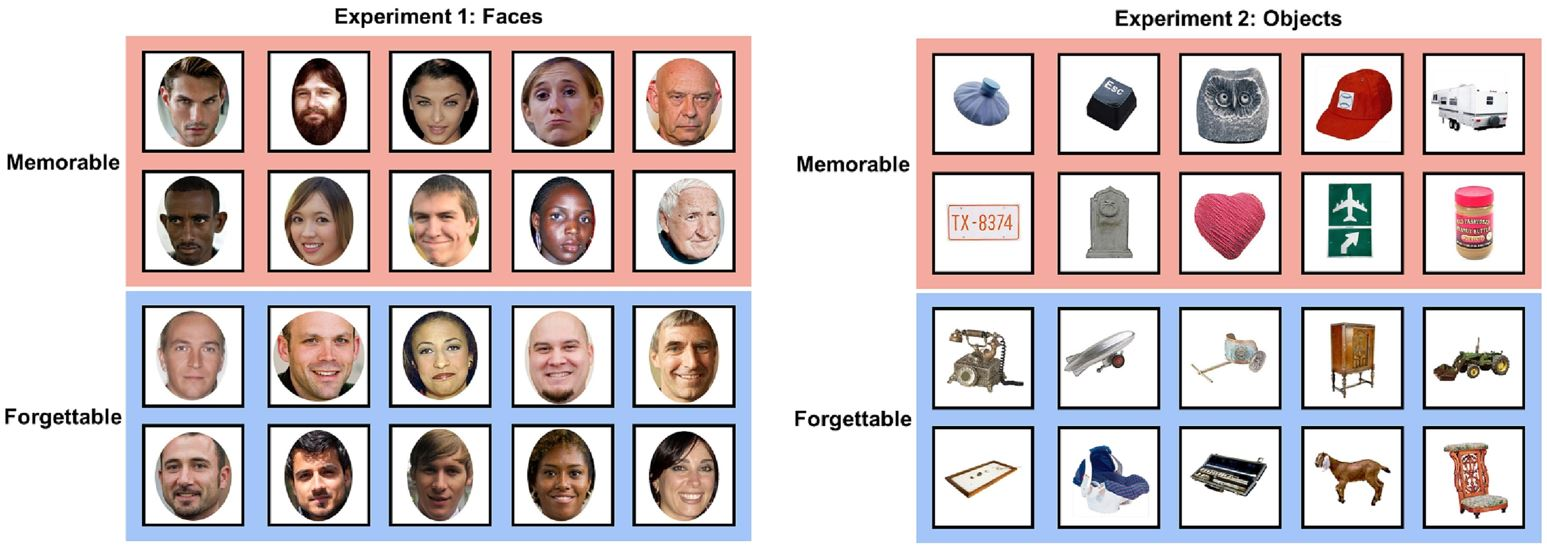
\includegraphics{stim.jpg}
The researchers conducted two experiments to examine how memorability benefits emerge by manipulating the stimulus memorability, set size, and degree of competition among stimuli as participants encoded them in the context of a working memory task. Subsequently, their memory for the encoded stimuli was tested in a VLTM task.
Specifically, in Experiment 1, they first selected the top 468 memorable face images and the top 468 forgettable face images from \href{see\%20Fig.\%201}{Bainbridge, Isola, and Oliva (2013)}.
In Experiment 2, they first selected the top 234 memorable object images and the top 234 forgettable object images from \href{see\%20Fig.\%201}{Saito, Kolisnyk, and Fukuda (2023)}.
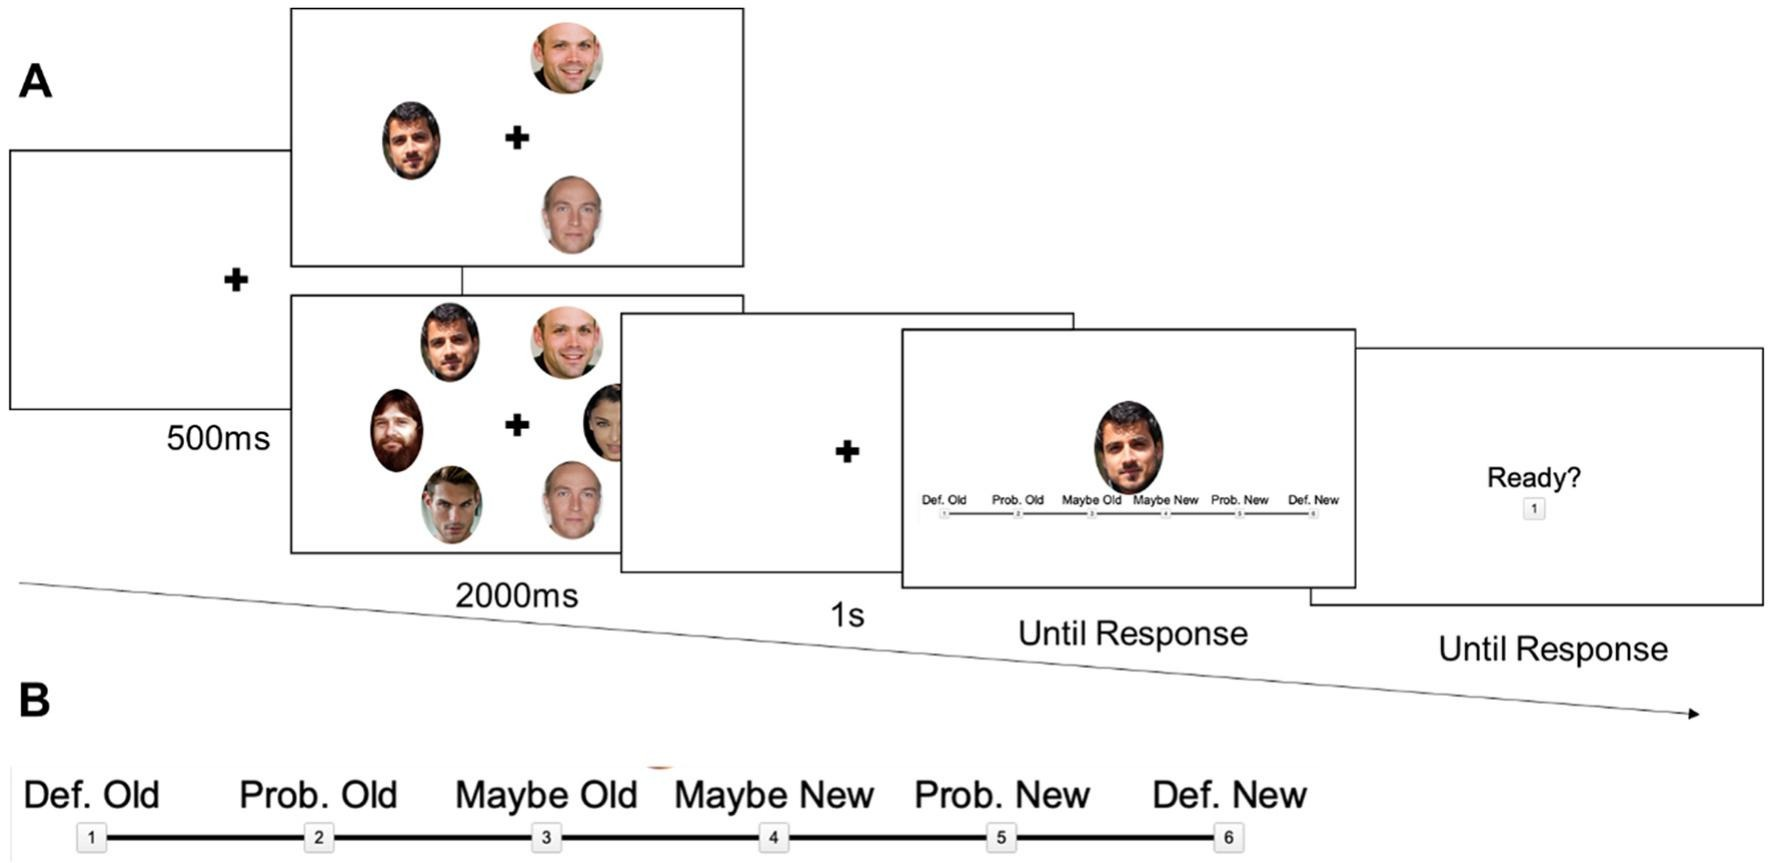
\includegraphics{vwm_task.jpg}
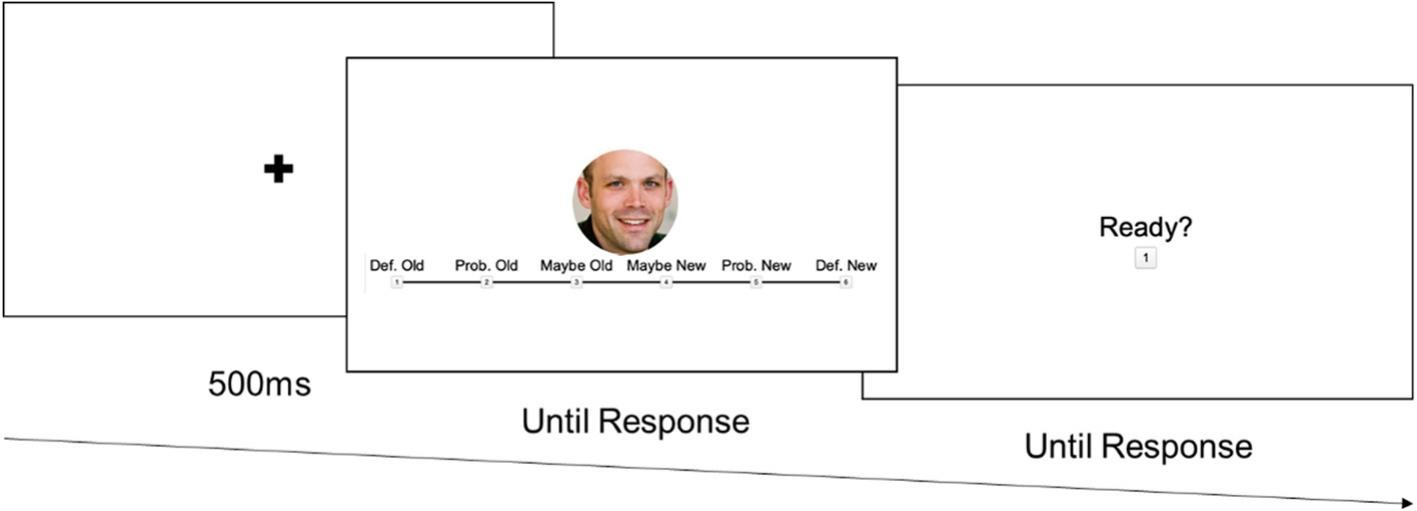
\includegraphics{VLTM_task.jpg}

\hypertarget{apparatus}{%
\subsection{Apparatus}\label{apparatus}}

The experiments were programmed and run using Inquisit 6 (Inquisit 6, 2020). Since the experiments were conducted online, the computers and monitors participants used were variable. Thus, the size of the stimuli was adjusted according to the monitor size of the participants' computers. More precisely, each stimulus was presented within an imaginary square whose side was 12\% the size of the shorter side of their computer monitors.

\hypertarget{data-analysis}{%
\subsection{Data analysis}\label{data-analysis}}

To confirm that VWM performance predicted VLTM performance, researchers conducted a series of correlational analyses between VWM and VLTM performance. To quantify memory performance using the same metric for both VWM and VLTM recognition tasks, they used the area under the receiver operating characteristic curves (AUC). The receiver operating characteristic curve is drawn by plotting the cumulative hit rate (the proportion of ``old'' responses when the stimulus is old) on the y-axis against the cumulative false alarm rate (the proportion of ``old'' responses when the stimulus is new) on the x-axis from the highest confidence old response (Definitely Old) to the lowest confidence old response (or the highest confidence new response (Definitely New)). The AUC will equal 1 when participants recognized all the encoded information with highest confidence (Definitely Old) and rejected all the new information with highest confidence (Definitely New). On the other hand, when participants cannot discriminate old from new information at all, the AUC will be equal to 0.5.

To investigate the efficiency and competitiveness hypotheses, they conducted a series of repeated measures ANOVAs examining the differential impacts of Array Type and Memorability on AUC for both VWM and VLTM.

To compute the proportion with which the amount of information in VWM is retained in VLTM, they defined the memory ``stickiness'' as (AUC for VLTM task -- 0.5) / (AUC for VWM recognition task -- 0.5).

To investigate the stickiness hypothesis in the context of storage efficiency, they conducted a series of repeated measures ANOVAs examining the differential impacts of Array Type and Memorability on memory stickiness.

\hypertarget{results}{%
\subsection{Results}\label{results}}

In the VWM task, performance was better for memorable stimuli compared to forgettable stimuli, supporting the efficiency hypothesis.
In addition, the researchers found that when in direct competition, memorable stimuli were also better at attracting limited VWM resources than forgettable stimuli, supporting the competitiveness hypothesis. However, only the efficiency advantage translated to a performance benefit in VLTM.
Lastly, they found that memorable stimuli were less likely to be forgotten after they passed through the encoding bottleneck imposed by VWM, supporting the ``stickiness'' hypothesis.
Thus, their results demonstrate that the memorability benefit develops across multiple cognitive processes.

\begin{verbatim}
##    Length     Class      Mode 
##      6681 character character
\end{verbatim}

\hypertarget{reproduction-procedure}{%
\section{Reproduction Procedure}\label{reproduction-procedure}}

Firstly, we trim the raw data and save them separately for further analysis.
Secondly, we conduct correlation and regression analysis to verify the prediction relationship between VWM performance and VLTM performance.
Thirdly, we conduct 2 (ArrayType: Pure 3 and Pure 6) × 2(Memorability: Memorable and Forgettable) repeated measures ANOVA on AUC to test the efficiency hypothesis. Similarly, we conduct 2 (ArrayType: Pure 6 and Mixed 6) × 2(Memorability: Memorable and Forgettable) repeated measures ANOVA on AUC to test the competitive hypothesis.
Fourthly, 2 (ArrayType: Pure 3 and Pure 6) × 2(Memorability: Memorable and Forgettable) rm ANOVA on stickiness and 2 (ArrayType: Mixed 6 and Pure 6) × 2(Memorability: Memorable and Forgettable) rm ANOVA on stickiness are conducted to test the stickiness hypothesis.
Importantly, given that the demographic information is not included in the raw data, the descriptive statistics results are not presented.
We used R (Version 4.2.3; R Core Team, 2023) and the R-packages \emph{bayestestR} (Version 0.13.1; Makowski, Ben-Shachar, \& Lüdecke, 2019), \emph{bruceR} (Version 0.8.10; Bao, 2023), \emph{dplyr} (Version 1.1.2; Wickham, François, Henry, Müller, \& Vaughan, 2023), \emph{ggplot2} (Version 3.4.2; Wickham, 2016), \emph{papaja} (Version 0.1.1.9001; Aust \& Barth, 2022), \emph{patchwork} (Version 1.1.2; Pedersen, 2022), and \emph{tidyr} (Version 1.3.0; Wickham, Vaughan, \& Girlich, 2023) for all our analyses. The results will be reported below.

\hypertarget{reproduction-results}{%
\section{Reproduction Results}\label{reproduction-results}}

\hypertarget{vwm-performance-predicts-vltm-performance}{%
\subsection{VWM performance predicts VLTM performance}\label{vwm-performance-predicts-vltm-performance}}

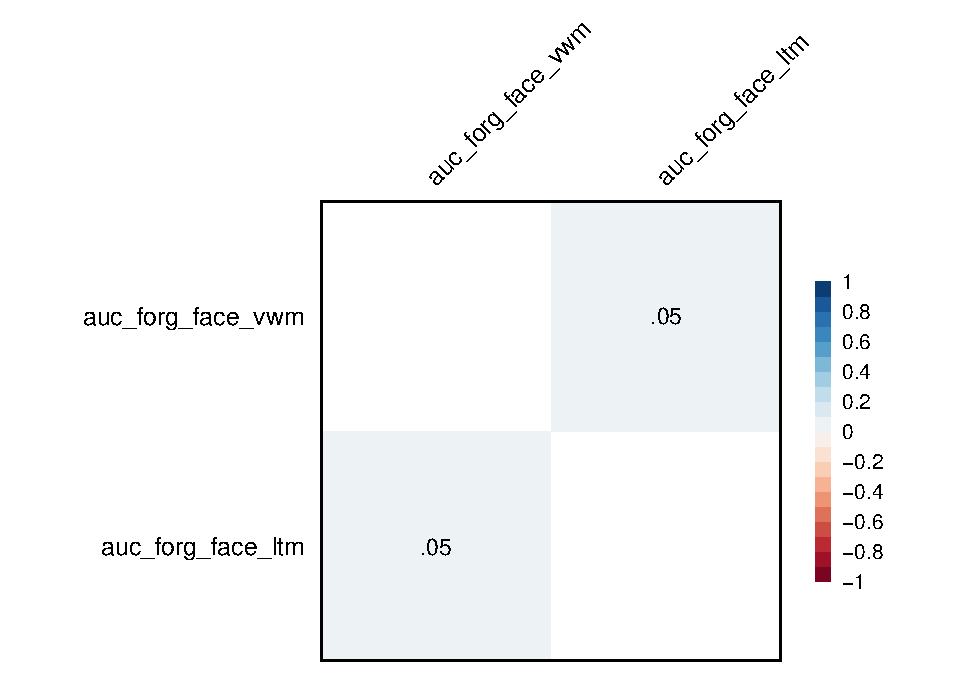
\includegraphics{Script_Re_Greer_2023_group1Rock_2023_files/figure-latex/plot-1.pdf}

\begin{verbatim}
## Correlation matrix is displayed in the RStudio `Plots` Pane.
## 
## Pearson's r and 95% confidence intervals:
## ─────────────────────────────────────────────────────────────────────
##                                         r      [95% CI]     p       N
## ─────────────────────────────────────────────────────────────────────
## auc_forg_face_vwm-auc_forg_face_ltm  0.05 [-0.11, 0.21]  .517     156
## ─────────────────────────────────────────────────────────────────────
\end{verbatim}

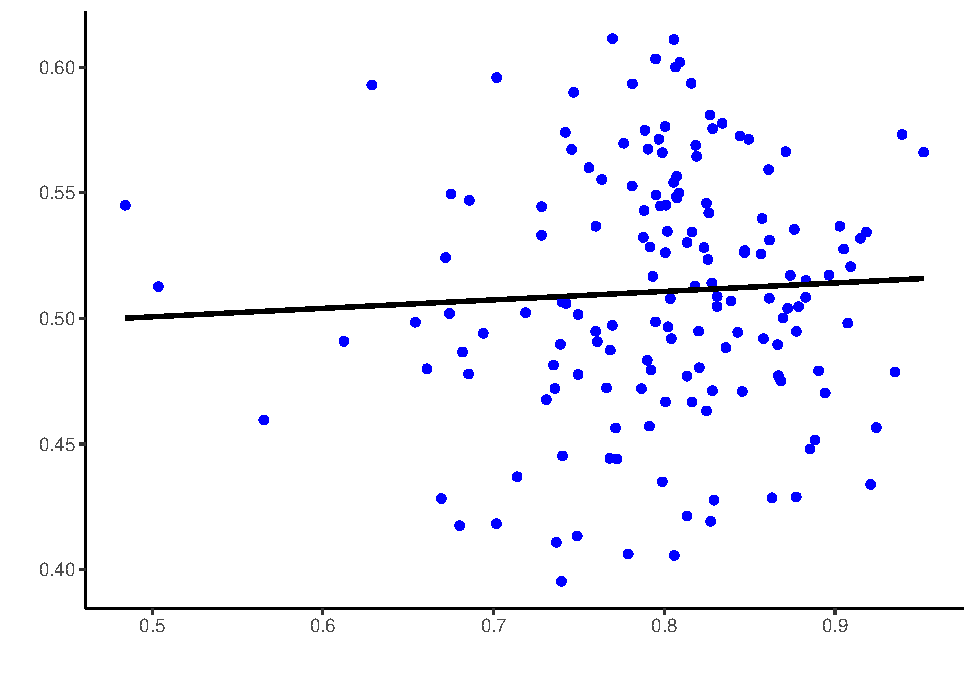
\includegraphics{Script_Re_Greer_2023_group1Rock_2023_files/figure-latex/plot-2.pdf}

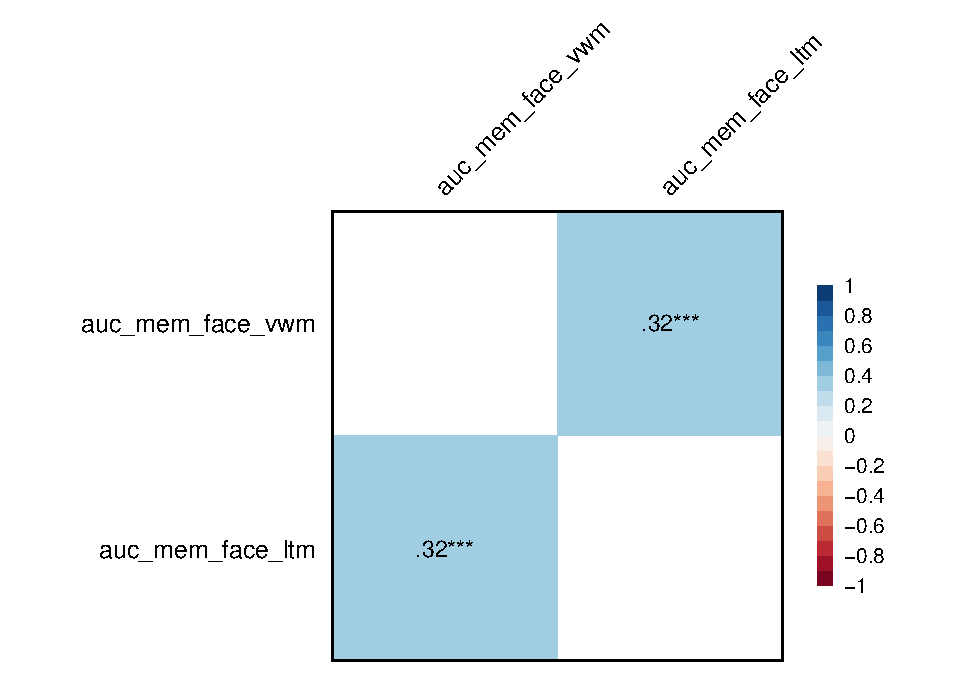
\includegraphics{Script_Re_Greer_2023_group1Rock_2023_files/figure-latex/unnamed-chunk-3-1.pdf}

\begin{verbatim}
## Correlation matrix is displayed in the RStudio `Plots` Pane.
## 
## Pearson's r and 95% confidence intervals:
## ──────────────────────────────────────────────────────────────────
##                                       r     [95% CI]     p       N
## ──────────────────────────────────────────────────────────────────
## auc_mem_face_vwm-auc_mem_face_ltm  0.32 [0.17, 0.46] <.001 *** 156
## ──────────────────────────────────────────────────────────────────
\end{verbatim}

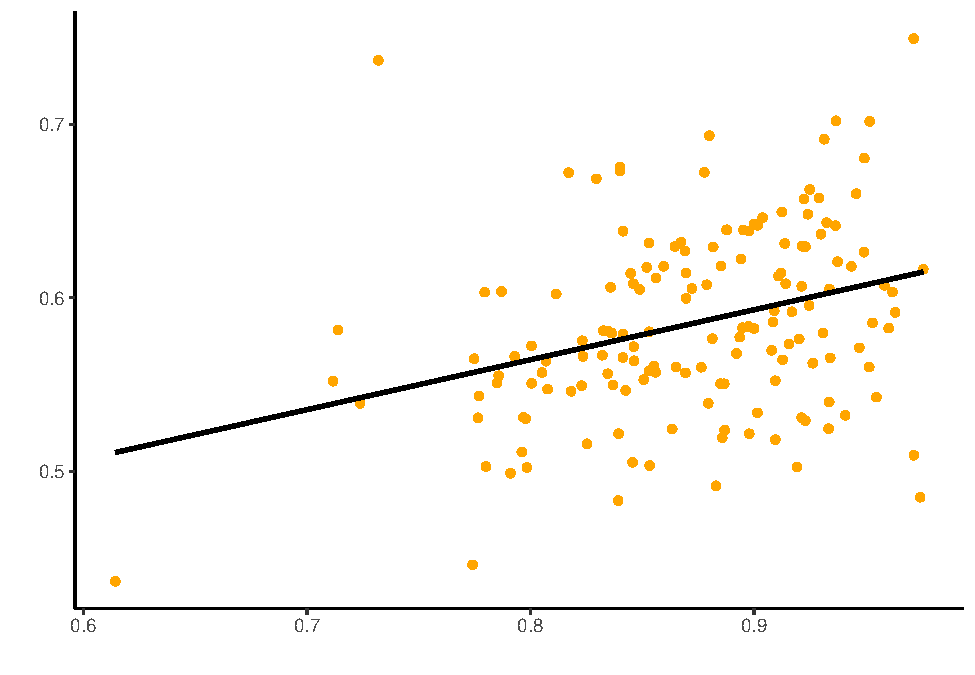
\includegraphics{Script_Re_Greer_2023_group1Rock_2023_files/figure-latex/unnamed-chunk-4-1.pdf}
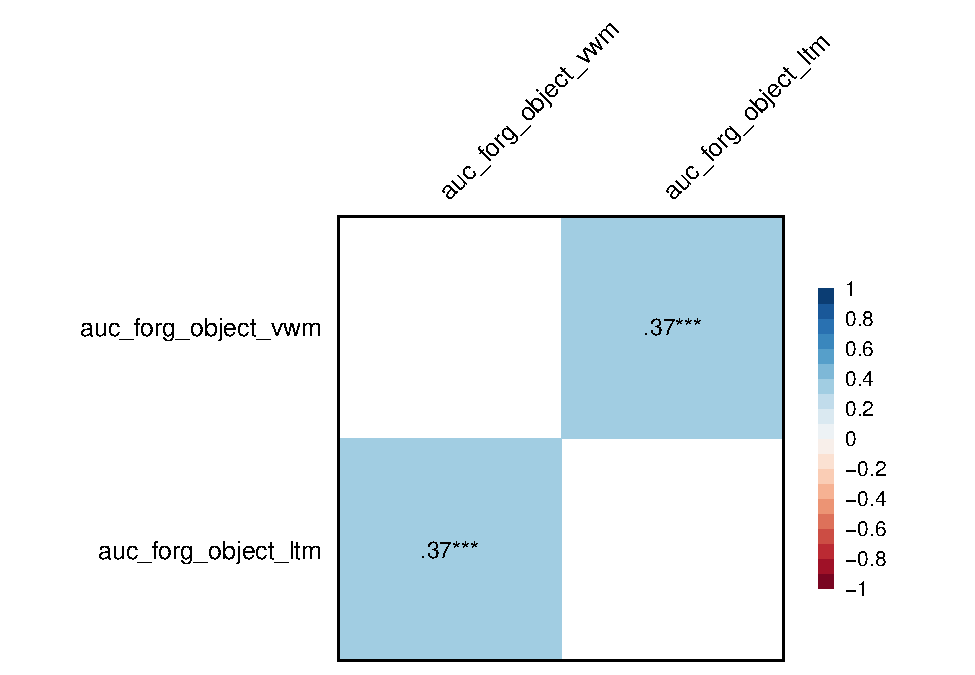
\includegraphics{Script_Re_Greer_2023_group1Rock_2023_files/figure-latex/unnamed-chunk-5-1.pdf}

\begin{verbatim}
## Correlation matrix is displayed in the RStudio `Plots` Pane.
## 
## Pearson's r and 95% confidence intervals:
## ────────────────────────────────────────────────────────────────────────
##                                             r     [95% CI]     p       N
## ────────────────────────────────────────────────────────────────────────
## auc_forg_object_vwm-auc_forg_object_ltm  0.37 [0.23, 0.50] <.001 *** 156
## ────────────────────────────────────────────────────────────────────────
\end{verbatim}

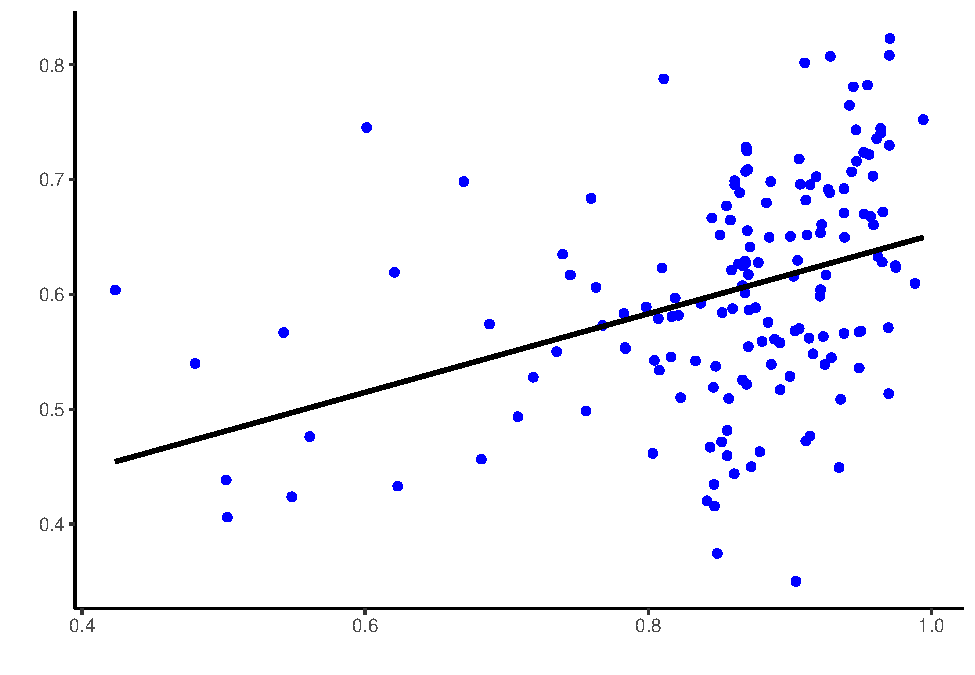
\includegraphics{Script_Re_Greer_2023_group1Rock_2023_files/figure-latex/unnamed-chunk-6-1.pdf}
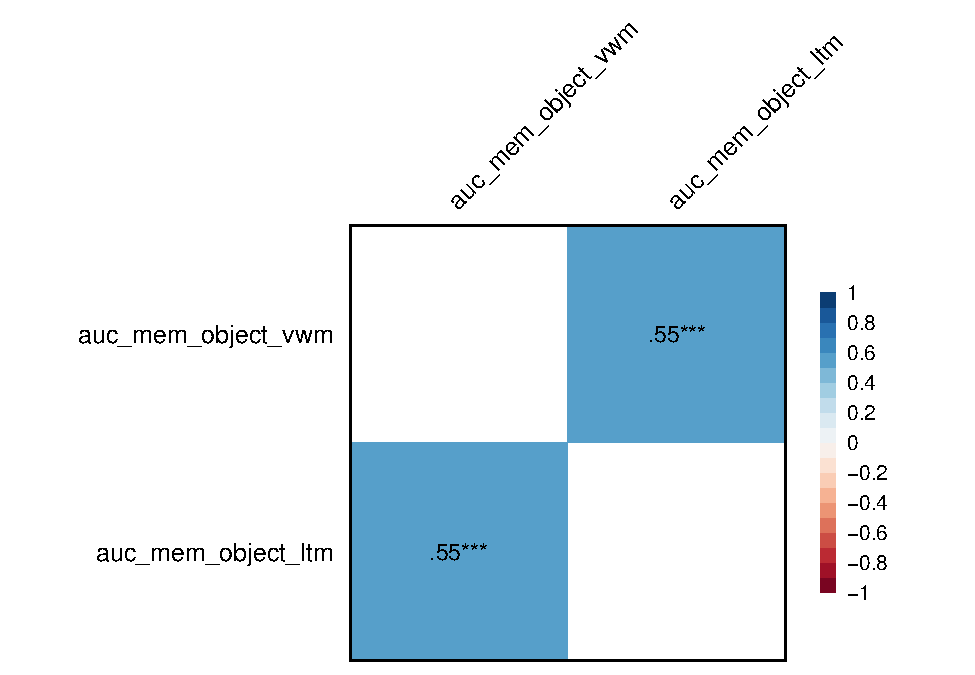
\includegraphics{Script_Re_Greer_2023_group1Rock_2023_files/figure-latex/unnamed-chunk-7-1.pdf}

\begin{verbatim}
## Correlation matrix is displayed in the RStudio `Plots` Pane.
## 
## Pearson's r and 95% confidence intervals:
## ──────────────────────────────────────────────────────────────────────
##                                           r     [95% CI]     p       N
## ──────────────────────────────────────────────────────────────────────
## auc_mem_object_vwm-auc_mem_object_ltm  0.55 [0.43, 0.65] <.001 *** 156
## ──────────────────────────────────────────────────────────────────────
\end{verbatim}

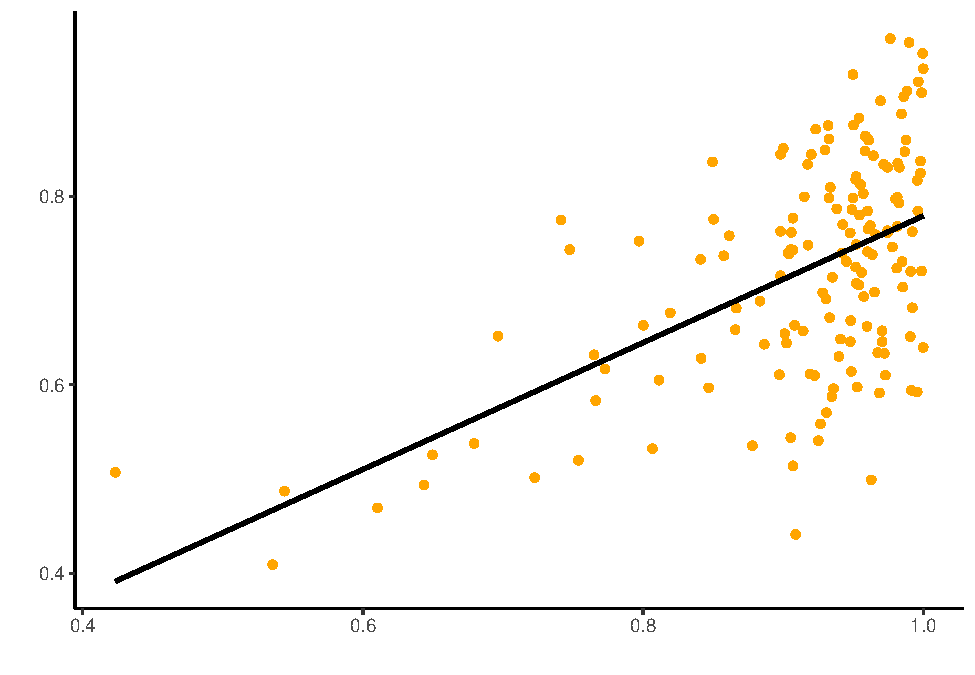
\includegraphics{Script_Re_Greer_2023_group1Rock_2023_files/figure-latex/unnamed-chunk-8-1.pdf}

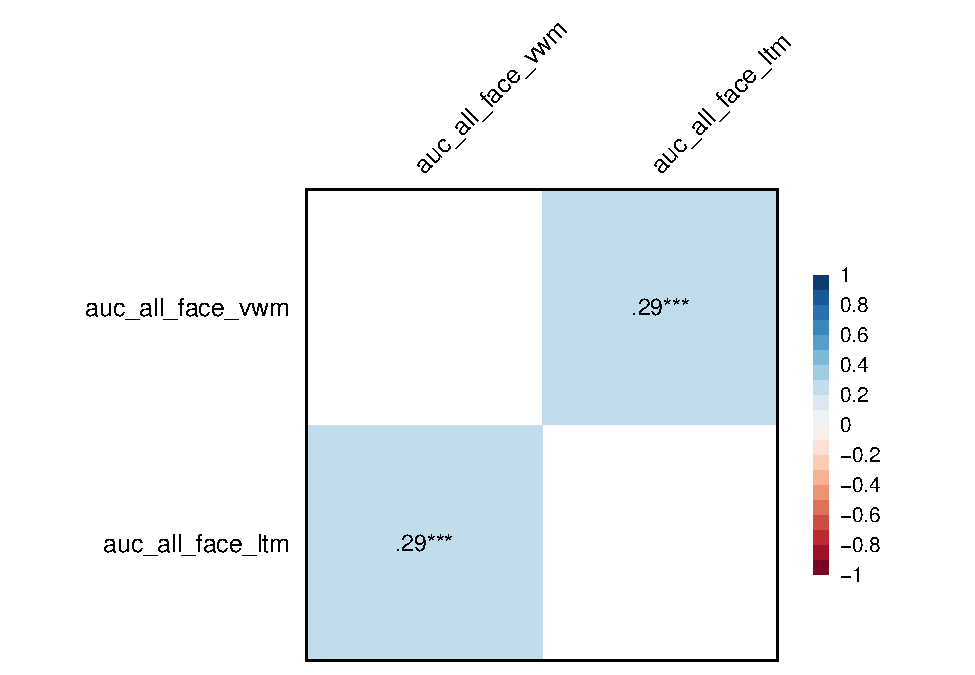
\includegraphics{Script_Re_Greer_2023_group1Rock_2023_files/figure-latex/unnamed-chunk-10-1.pdf}

\begin{verbatim}
## Correlation matrix is displayed in the RStudio `Plots` Pane.
## 
## Pearson's r and 95% confidence intervals:
## ──────────────────────────────────────────────────────────────────
##                                       r     [95% CI]     p       N
## ──────────────────────────────────────────────────────────────────
## auc_all_face_vwm-auc_all_face_ltm  0.29 [0.14, 0.43] <.001 *** 156
## ──────────────────────────────────────────────────────────────────
\end{verbatim}

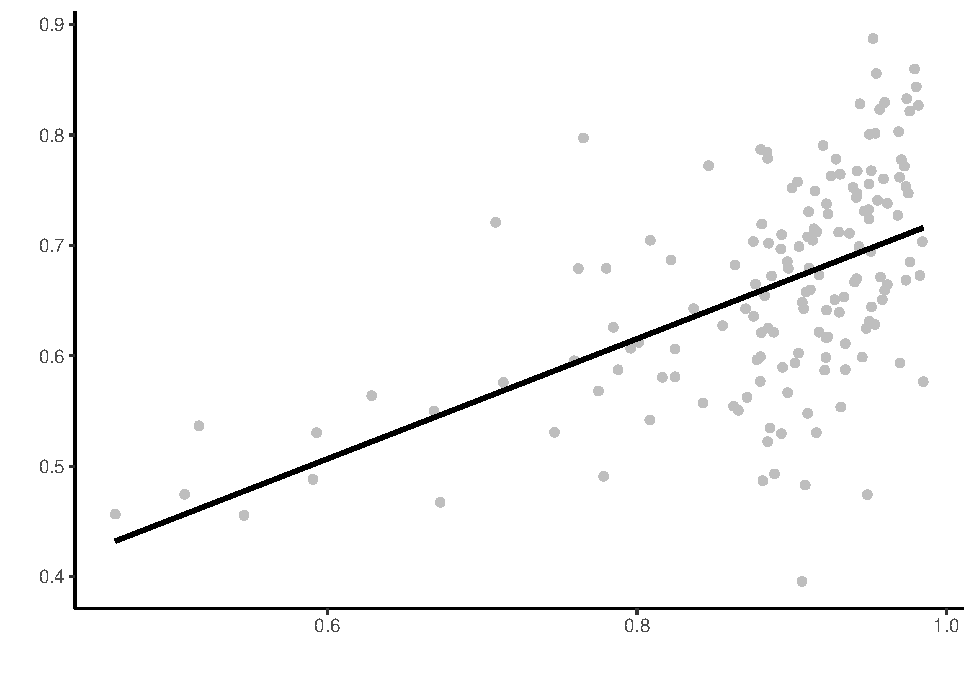
\includegraphics{Script_Re_Greer_2023_group1Rock_2023_files/figure-latex/unnamed-chunk-11-1.pdf}

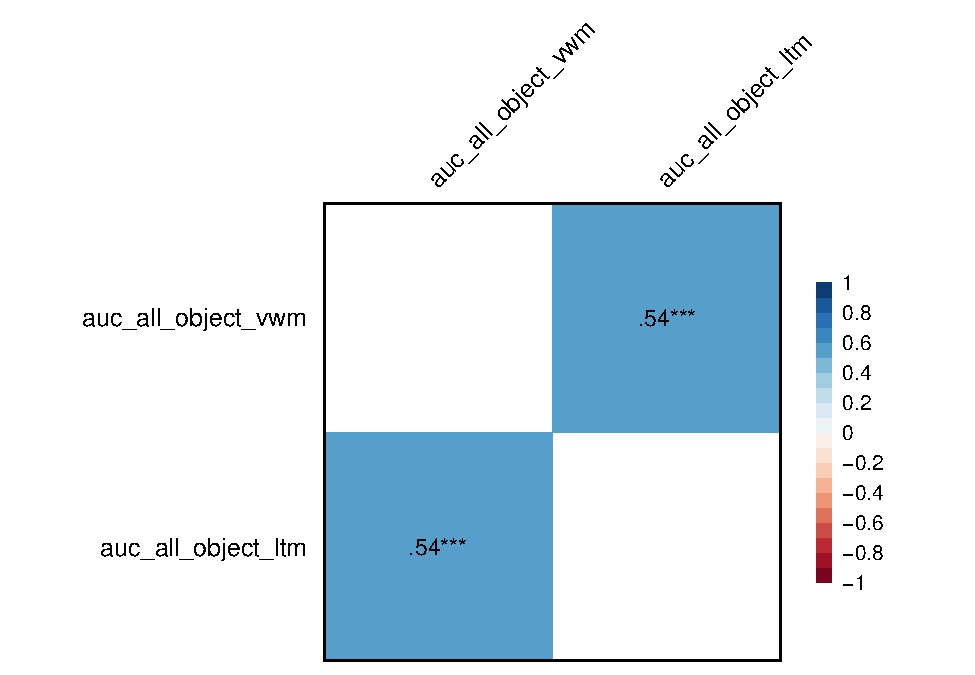
\includegraphics{Script_Re_Greer_2023_group1Rock_2023_files/figure-latex/unnamed-chunk-12-1.pdf}

\begin{verbatim}
## Correlation matrix is displayed in the RStudio `Plots` Pane.
## 
## Pearson's r and 95% confidence intervals:
## ──────────────────────────────────────────────────────────────────────
##                                           r     [95% CI]     p       N
## ──────────────────────────────────────────────────────────────────────
## auc_all_object_vwm-auc_all_object_ltm  0.54 [0.41, 0.64] <.001 *** 156
## ──────────────────────────────────────────────────────────────────────
\end{verbatim}

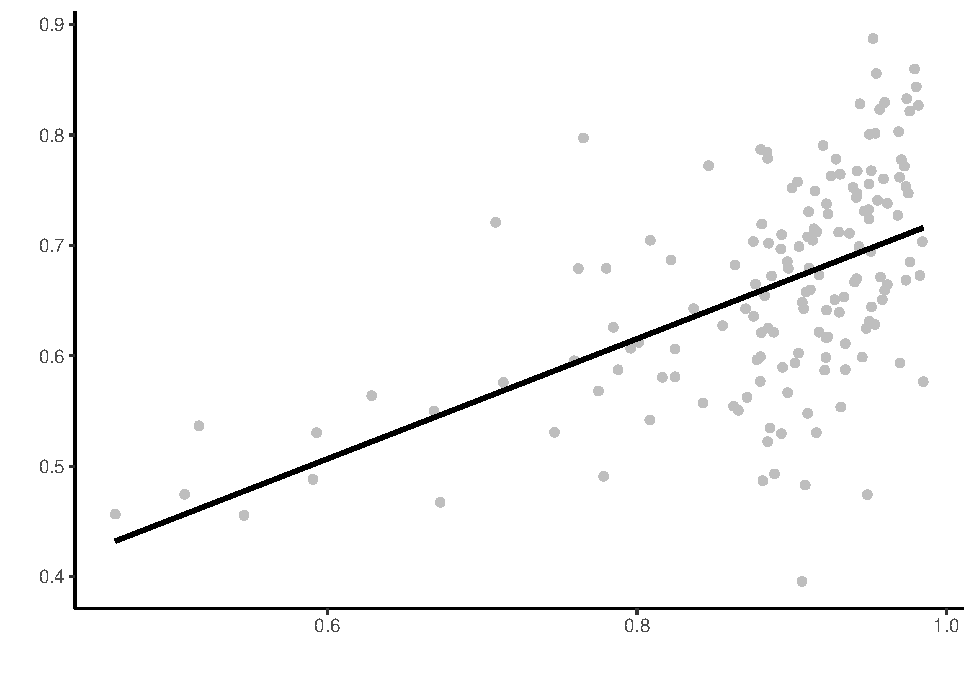
\includegraphics{Script_Re_Greer_2023_group1Rock_2023_files/figure-latex/unnamed-chunk-13-1.pdf}

\hypertarget{testing-the-efficiency-hypothesis-memorable-stimuli-are-more-efficiently-represented-in-vwm-than-forgettable-stimuli}{%
\subsection{Testing the efficiency hypothesis: memorable stimuli are more efficiently represented in VWM than forgettable stimuli}\label{testing-the-efficiency-hypothesis-memorable-stimuli-are-more-efficiently-represented-in-vwm-than-forgettable-stimuli}}

\begin{verbatim}
##  [1] "------ EMMEANS (effect = \"A_\") ------"                                           
##  [2] ""                                                                                  
##  [3] "Joint Tests of \"A_\":"                                                            
##  [4] "──────────────────────────────────────────────────────────"                        
##  [5] " Effect \"B_\" df1 df2       F     p     η²p [90% CI of η²p]"                      
##  [6] "──────────────────────────────────────────────────────────"                        
##  [7] "     A_ Forg   1 155 552.669 <.001 ***   .781 [.735, .816]"                        
##  [8] "     A_ Mem    1 155 433.024 <.001 ***   .736 [.682, .778]"                        
##  [9] "──────────────────────────────────────────────────────────"                        
## [10] "Note. Simple effects of repeated measures with 3 or more levels"                   
## [11] "are different from the results obtained with SPSS MANOVA syntax."                  
## [12] ""                                                                                  
## [13] "Estimated Marginal Means of \"A_\":"                                               
## [14] "────────────────────────────────────────"                                          
## [15] " \"A_\" \"B_\" Mean [95% CI of Mean]    S.E."                                      
## [16] "────────────────────────────────────────"                                          
## [17] " SS3. Forg  0.892 [0.879, 0.905] (0.006)"                                          
## [18] " SS6. Forg  0.737 [0.721, 0.752] (0.008)"                                          
## [19] " SS3. Mem   0.941 [0.933, 0.950] (0.004)"                                          
## [20] " SS6. Mem   0.812 [0.799, 0.826] (0.007)"                                          
## [21] "────────────────────────────────────────"                                          
## [22] ""                                                                                  
## [23] "Pairwise Comparisons of \"A_\":"                                                   
## [24] "────────────────────────────────────────────────────────────────────────────────"  
## [25] "    Contrast \"B_\" Estimate    S.E.  df       t     p     Cohen’s d [95% CI of d]"
## [26] "────────────────────────────────────────────────────────────────────────────────"  
## [27] " SS6. - SS3. Forg   -0.155 (0.007) 155 -23.509 <.001 *** -1.844 [-1.999, -1.689]"  
## [28] " SS6. - SS3. Mem    -0.129 (0.006) 155 -20.809 <.001 *** -1.531 [-1.676, -1.385]"  
## [29] "────────────────────────────────────────────────────────────────────────────────"  
## [30] "Pooled SD for computing Cohen’s d: 0.084"                                          
## [31] "No need to adjust p values."                                                       
## [32] ""                                                                                  
## [33] "Disclaimer:"                                                                       
## [34] "By default, pooled SD is Root Mean Square Error (RMSE)."                           
## [35] "There is much disagreement on how to compute Cohen’s d."                           
## [36] "You are completely responsible for setting `sd.pooled`."                           
## [37] "You might also use `effectsize::t_to_d()` to compute d."                           
## [38] ""
\end{verbatim}

\begin{verbatim}
##  [1] ""                                                                                       
##  [2] "====== ANOVA (Within-Subjects Design) ======"                                           
##  [3] ""                                                                                       
##  [4] "Descriptives:"                                                                          
##  [5] "────────────────────────────"                                                           
##  [6] " \"A_\" \"B_\"  Mean    S.D.   n"                                                       
##  [7] "────────────────────────────"                                                           
##  [8] " SS3. Forg 0.527 (0.067) 156"                                                           
##  [9] " SS3. Mem  0.640 (0.076) 156"                                                           
## [10] " SS6. Forg 0.502 (0.070) 156"                                                           
## [11] " SS6. Mem  0.554 (0.077) 156"                                                           
## [12] "────────────────────────────"                                                           
## [13] "Total sample size: N = 156"                                                             
## [14] ""                                                                                       
## [15] "ANOVA Table:"                                                                           
## [16] "Dependent variable(s):      A_SS3&B_Forg, A_SS3&B_Mem, A_SS6&B_Forg, A_SS6&B_Mem"       
## [17] "Between-subjects factor(s): –"                                                          
## [18] "Within-subjects factor(s):  A_, B_"                                                     
## [19] "Covariate(s):               –"                                                          
## [20] "───────────────────────────────────────────────────────────────────────"                
## [21] "            MS   MSE df1 df2       F     p     η²p [90% CI of η²p]  η²G"                
## [22] "───────────────────────────────────────────────────────────────────────"                
## [23] "A_       0.474 0.004   1 155 124.695 <.001 ***   .446 [.353, .525] .127"                
## [24] "B_       1.068 0.005   1 155 203.842 <.001 ***   .568 [.488, .634] .246"                
## [25] "A_ * B_  0.147 0.004   1 155  38.096 <.001 ***   .197 [.112, .287] .043"                
## [26] "───────────────────────────────────────────────────────────────────────"                
## [27] "MSE = mean square error (the residual variance of the linear model)"                    
## [28] "η²p = partial eta-squared = SS / (SS + SSE) = F * df1 / (F * df1 + df2)"                
## [29] "ω²p = partial omega-squared = (F - 1) * df1 / (F * df1 + df2 + 1)"                      
## [30] "η²G = generalized eta-squared (see Olejnik & Algina, 2003)"                             
## [31] "Cohen’s f² = η²p / (1 - η²p)"                                                           
## [32] ""                                                                                       
## [33] "Levene’s Test for Homogeneity of Variance:"                                             
## [34] "No between-subjects factors. No need to do the Levene’s test."                          
## [35] ""                                                                                       
## [36] "Mauchly’s Test of Sphericity:"                                                          
## [37] "The repeated measures have only two levels. The assumption of sphericity is always met."
## [38] ""
\end{verbatim}

\begin{verbatim}
##  [1] "------ EMMEANS (effect = \"A_\") ------"                                           
##  [2] ""                                                                                  
##  [3] "Joint Tests of \"A_\":"                                                            
##  [4] "──────────────────────────────────────────────────────────"                        
##  [5] " Effect \"B_\" df1 df2       F     p     η²p [90% CI of η²p]"                      
##  [6] "──────────────────────────────────────────────────────────"                        
##  [7] "     A_ Forg   1 155  12.837 <.001 ***   .076 [.023, .151]"                        
##  [8] "     A_ Mem    1 155 141.691 <.001 ***   .478 [.388, .554]"                        
##  [9] "──────────────────────────────────────────────────────────"                        
## [10] "Note. Simple effects of repeated measures with 3 or more levels"                   
## [11] "are different from the results obtained with SPSS MANOVA syntax."                  
## [12] ""                                                                                  
## [13] "Estimated Marginal Means of \"A_\":"                                               
## [14] "────────────────────────────────────────"                                          
## [15] " \"A_\" \"B_\" Mean [95% CI of Mean]    S.E."                                      
## [16] "────────────────────────────────────────"                                          
## [17] " SS3. Forg  0.527 [0.516, 0.537] (0.005)"                                          
## [18] " SS6. Forg  0.502 [0.491, 0.513] (0.006)"                                          
## [19] " SS3. Mem   0.640 [0.628, 0.652] (0.006)"                                          
## [20] " SS6. Mem   0.554 [0.542, 0.566] (0.006)"                                          
## [21] "────────────────────────────────────────"                                          
## [22] ""                                                                                  
## [23] "Pairwise Comparisons of \"A_\":"                                                   
## [24] "────────────────────────────────────────────────────────────────────────────────"  
## [25] "    Contrast \"B_\" Estimate    S.E.  df       t     p     Cohen’s d [95% CI of d]"
## [26] "────────────────────────────────────────────────────────────────────────────────"  
## [27] " SS6. - SS3. Forg   -0.024 (0.007) 155  -3.583 <.001 *** -0.263 [-0.408, -0.118]"  
## [28] " SS6. - SS3. Mem    -0.086 (0.007) 155 -11.903 <.001 *** -0.926 [-1.079, -0.772]"  
## [29] "────────────────────────────────────────────────────────────────────────────────"  
## [30] "Pooled SD for computing Cohen’s d: 0.093"                                          
## [31] "No need to adjust p values."                                                       
## [32] ""                                                                                  
## [33] "Disclaimer:"                                                                       
## [34] "By default, pooled SD is Root Mean Square Error (RMSE)."                           
## [35] "There is much disagreement on how to compute Cohen’s d."                           
## [36] "You are completely responsible for setting `sd.pooled`."                           
## [37] "You might also use `effectsize::t_to_d()` to compute d."                           
## [38] ""
\end{verbatim}

\begin{verbatim}
##  [1] ""                                                                                       
##  [2] "====== ANOVA (Within-Subjects Design) ======"                                           
##  [3] ""                                                                                       
##  [4] "Descriptives:"                                                                          
##  [5] "────────────────────────────"                                                           
##  [6] " \"A_\" \"B_\"  Mean    S.D.   n"                                                       
##  [7] "────────────────────────────"                                                           
##  [8] " SS3. Forg 0.678 (0.151) 156"                                                           
##  [9] " SS3. Mem  0.813 (0.151) 156"                                                           
## [10] " SS6. Forg 0.566 (0.110) 156"                                                           
## [11] " SS6. Mem  0.678 (0.122) 156"                                                           
## [12] "────────────────────────────"                                                           
## [13] "Total sample size: N = 156"                                                             
## [14] ""                                                                                       
## [15] "ANOVA Table:"                                                                           
## [16] "Dependent variable(s):      A_SS3&B_Forg, A_SS3&B_Mem, A_SS6&B_Forg, A_SS6&B_Mem"       
## [17] "Between-subjects factor(s): –"                                                          
## [18] "Within-subjects factor(s):  A_, B_"                                                     
## [19] "Covariate(s):               –"                                                          
## [20] "───────────────────────────────────────────────────────────────────────"                
## [21] "            MS   MSE df1 df2       F     p     η²p [90% CI of η²p]  η²G"                
## [22] "───────────────────────────────────────────────────────────────────────"                
## [23] "A_       2.369 0.010   1 155 246.658 <.001 ***   .614 [.540, .674] .174"                
## [24] "B_       2.386 0.011   1 155 219.761 <.001 ***   .586 [.508, .650] .175"                
## [25] "A_ * B_  0.021 0.007   1 155   2.882  .092 .     .018 [.000, .067] .002"                
## [26] "───────────────────────────────────────────────────────────────────────"                
## [27] "MSE = mean square error (the residual variance of the linear model)"                    
## [28] "η²p = partial eta-squared = SS / (SS + SSE) = F * df1 / (F * df1 + df2)"                
## [29] "ω²p = partial omega-squared = (F - 1) * df1 / (F * df1 + df2 + 1)"                      
## [30] "η²G = generalized eta-squared (see Olejnik & Algina, 2003)"                             
## [31] "Cohen’s f² = η²p / (1 - η²p)"                                                           
## [32] ""                                                                                       
## [33] "Levene’s Test for Homogeneity of Variance:"                                             
## [34] "No between-subjects factors. No need to do the Levene’s test."                          
## [35] ""                                                                                       
## [36] "Mauchly’s Test of Sphericity:"                                                          
## [37] "The repeated measures have only two levels. The assumption of sphericity is always met."
## [38] ""
\end{verbatim}

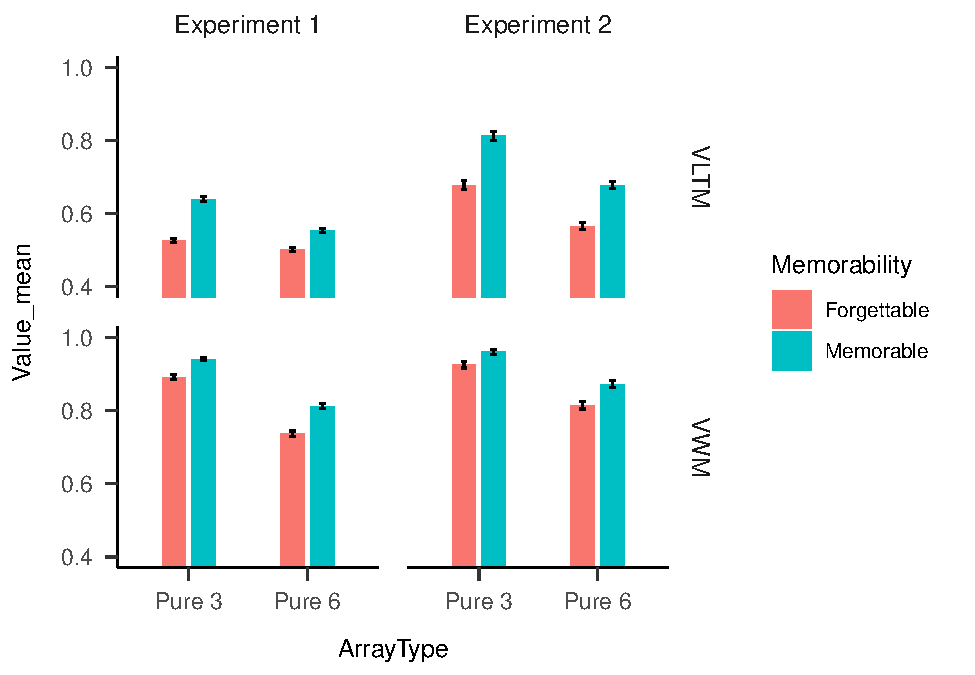
\includegraphics{Script_Re_Greer_2023_group1Rock_2023_files/figure-latex/plot for efficiency hypothesis-1.pdf}

We use simple barplot for comparing with the paper result, but it is too simple to be informative, so we create another split violin plot.
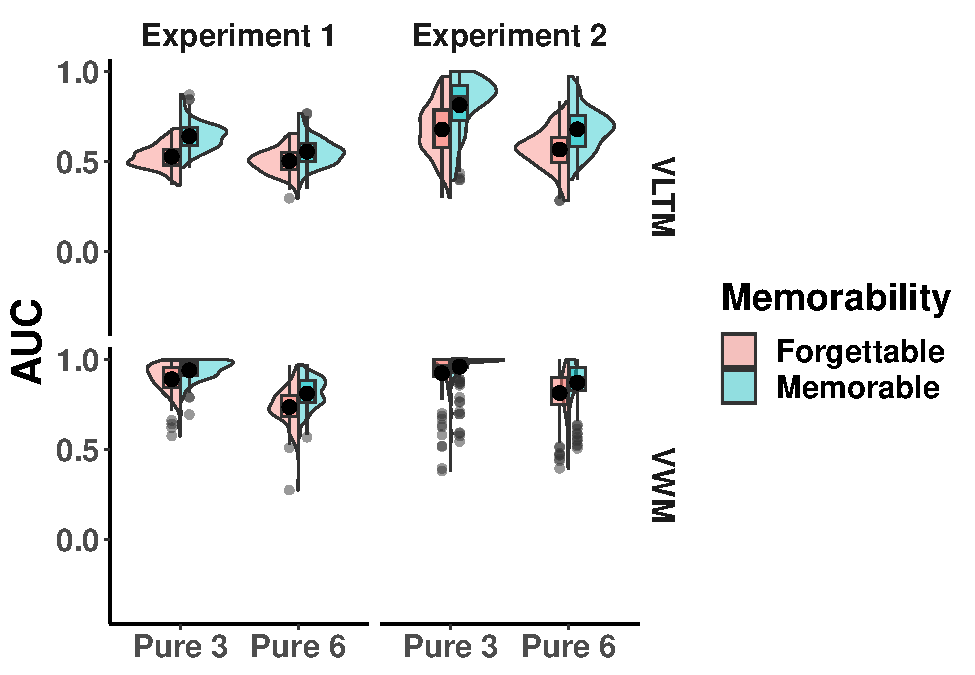
\includegraphics{Script_Re_Greer_2023_group1Rock_2023_files/figure-latex/Split violin plots for efficiency hypo-1.pdf}

\hypertarget{testing-the-competitiveness-hypothesis-memorable-stimuli-attract-more-vwm-resources-than-forgettable-stimuli}{%
\subsection{Testing the competitiveness hypothesis: memorable stimuli attract more VWM resources than forgettable stimuli}\label{testing-the-competitiveness-hypothesis-memorable-stimuli-attract-more-vwm-resources-than-forgettable-stimuli}}

\begin{verbatim}
##  [1] ""                                                                                       
##  [2] "====== ANOVA (Within-Subjects Design) ======"                                           
##  [3] ""                                                                                       
##  [4] "Descriptives:"                                                                          
##  [5] "──────────────────────────────"                                                         
##  [6] "   \"A_\" \"B_\"  Mean    S.D.   n"                                                     
##  [7] "──────────────────────────────"                                                         
##  [8] " Mixed. Forg 0.725 (0.092) 156"                                                         
##  [9] " Mixed. Mem  0.836 (0.085) 156"                                                         
## [10] " SS6.   Forg 0.737 (0.099) 156"                                                         
## [11] " SS6.   Mem  0.812 (0.084) 156"                                                         
## [12] "──────────────────────────────"                                                         
## [13] "Total sample size: N = 156"                                                             
## [14] ""                                                                                       
## [15] "ANOVA Table:"                                                                           
## [16] "Dependent variable(s):      A_Mixed&B_Forg, A_Mixed&B_Mem, A_SS6&B_Forg, A_SS6&B_Mem"   
## [17] "Between-subjects factor(s): –"                                                          
## [18] "Within-subjects factor(s):  A_, B_"                                                     
## [19] "Covariate(s):               –"                                                          
## [20] "───────────────────────────────────────────────────────────────────────"                
## [21] "            MS   MSE df1 df2       F     p     η²p [90% CI of η²p]  η²G"                
## [22] "───────────────────────────────────────────────────────────────────────"                
## [23] "A_       0.005 0.005   1 155   1.058  .305       .007 [.000, .044] .001"                
## [24] "B_       1.366 0.004   1 155 313.183 <.001 ***   .669 [.603, .721] .213"                
## [25] "A_ * B_  0.050 0.004   1 155  11.775 <.001 ***   .071 [.019, .144] .010"                
## [26] "───────────────────────────────────────────────────────────────────────"                
## [27] "MSE = mean square error (the residual variance of the linear model)"                    
## [28] "η²p = partial eta-squared = SS / (SS + SSE) = F * df1 / (F * df1 + df2)"                
## [29] "ω²p = partial omega-squared = (F - 1) * df1 / (F * df1 + df2 + 1)"                      
## [30] "η²G = generalized eta-squared (see Olejnik & Algina, 2003)"                             
## [31] "Cohen’s f² = η²p / (1 - η²p)"                                                           
## [32] ""                                                                                       
## [33] "Levene’s Test for Homogeneity of Variance:"                                             
## [34] "No between-subjects factors. No need to do the Levene’s test."                          
## [35] ""                                                                                       
## [36] "Mauchly’s Test of Sphericity:"                                                          
## [37] "The repeated measures have only two levels. The assumption of sphericity is always met."
## [38] ""
\end{verbatim}

\begin{verbatim}
##  [1] "------ EMMEANS (effect = \"A_\") ------"                                            
##  [2] ""                                                                                   
##  [3] "Joint Tests of \"A_\":"                                                             
##  [4] "─────────────────────────────────────────────────────────"                          
##  [5] " Effect \"B_\" df1 df2      F     p     η²p [90% CI of η²p]"                        
##  [6] "─────────────────────────────────────────────────────────"                          
##  [7] "     A_ Forg   1 155  2.228  .138       .014 [.000, .060]"                          
##  [8] "     A_ Mem    1 155 11.292 <.001 ***   .068 [.018, .140]"                          
##  [9] "─────────────────────────────────────────────────────────"                          
## [10] "Note. Simple effects of repeated measures with 3 or more levels"                    
## [11] "are different from the results obtained with SPSS MANOVA syntax."                   
## [12] ""                                                                                   
## [13] "Estimated Marginal Means of \"A_\":"                                                
## [14] "──────────────────────────────────────────"                                         
## [15] "   \"A_\" \"B_\" Mean [95% CI of Mean]    S.E."                                     
## [16] "──────────────────────────────────────────"                                         
## [17] " Mixed. Forg  0.725 [0.710, 0.739] (0.007)"                                         
## [18] " SS6.   Forg  0.737 [0.721, 0.752] (0.008)"                                         
## [19] " Mixed. Mem   0.836 [0.823, 0.849] (0.007)"                                         
## [20] " SS6.   Mem   0.812 [0.799, 0.826] (0.007)"                                         
## [21] "──────────────────────────────────────────"                                         
## [22] ""                                                                                   
## [23] "Pairwise Comparisons of \"A_\":"                                                    
## [24] "─────────────────────────────────────────────────────────────────────────────────"  
## [25] "      Contrast \"B_\" Estimate    S.E.  df      t     p     Cohen’s d [95% CI of d]"
## [26] "─────────────────────────────────────────────────────────────────────────────────"  
## [27] " SS6. - Mixed. Forg    0.012 (0.008) 155  1.493  .138      0.129 [-0.042,  0.299]"  
## [28] " SS6. - Mixed. Mem    -0.024 (0.007) 155 -3.360 <.001 *** -0.249 [-0.396, -0.103]"  
## [29] "─────────────────────────────────────────────────────────────────────────────────"  
## [30] "Pooled SD for computing Cohen’s d: 0.094"                                           
## [31] "No need to adjust p values."                                                        
## [32] ""                                                                                   
## [33] "Disclaimer:"                                                                        
## [34] "By default, pooled SD is Root Mean Square Error (RMSE)."                            
## [35] "There is much disagreement on how to compute Cohen’s d."                            
## [36] "You are completely responsible for setting `sd.pooled`."                            
## [37] "You might also use `effectsize::t_to_d()` to compute d."                            
## [38] ""
\end{verbatim}

\begin{verbatim}
##  [1] ""                                                                                       
##  [2] "====== ANOVA (Within-Subjects Design) ======"                                           
##  [3] ""                                                                                       
##  [4] "Descriptives:"                                                                          
##  [5] "──────────────────────────────"                                                         
##  [6] "   \"A_\" \"B_\"  Mean    S.D.   n"                                                     
##  [7] "──────────────────────────────"                                                         
##  [8] " Mixed. Forg 0.802 (0.130) 156"                                                         
##  [9] " Mixed. Mem  0.891 (0.132) 156"                                                         
## [10] " SS6.   Forg 0.815 (0.129) 156"                                                         
## [11] " SS6.   Mem  0.873 (0.114) 156"                                                         
## [12] "──────────────────────────────"                                                         
## [13] "Total sample size: N = 156"                                                             
## [14] ""                                                                                       
## [15] "ANOVA Table:"                                                                           
## [16] "Dependent variable(s):      A_Mixed&B_Forg, A_Mixed&B_Mem, A_SS6&B_Forg, A_SS6&B_Mem"   
## [17] "Between-subjects factor(s): –"                                                          
## [18] "Within-subjects factor(s):  A_, B_"                                                     
## [19] "Covariate(s):               –"                                                          
## [20] "───────────────────────────────────────────────────────────────────────"                
## [21] "            MS   MSE df1 df2       F     p     η²p [90% CI of η²p]  η²G"                
## [22] "───────────────────────────────────────────────────────────────────────"                
## [23] "A_       0.001 0.005   1 155   0.207  .650       .001 [.000, .026] .000"                
## [24] "B_       0.839 0.008   1 155 102.498 <.001 ***   .398 [.303, .482] .078"                
## [25] "A_ * B_  0.037 0.007   1 155   5.440  .021 *     .034 [.003, .093] .004"                
## [26] "───────────────────────────────────────────────────────────────────────"                
## [27] "MSE = mean square error (the residual variance of the linear model)"                    
## [28] "η²p = partial eta-squared = SS / (SS + SSE) = F * df1 / (F * df1 + df2)"                
## [29] "ω²p = partial omega-squared = (F - 1) * df1 / (F * df1 + df2 + 1)"                      
## [30] "η²G = generalized eta-squared (see Olejnik & Algina, 2003)"                             
## [31] "Cohen’s f² = η²p / (1 - η²p)"                                                           
## [32] ""                                                                                       
## [33] "Levene’s Test for Homogeneity of Variance:"                                             
## [34] "No between-subjects factors. No need to do the Levene’s test."                          
## [35] ""                                                                                       
## [36] "Mauchly’s Test of Sphericity:"                                                          
## [37] "The repeated measures have only two levels. The assumption of sphericity is always met."
## [38] ""
\end{verbatim}

\begin{verbatim}
##  [1] "------ EMMEANS (effect = \"A_\") ------"                                            
##  [2] ""                                                                                   
##  [3] "Joint Tests of \"A_\":"                                                             
##  [4] "────────────────────────────────────────────────────────"                           
##  [5] " Effect \"B_\" df1 df2     F     p     η²p [90% CI of η²p]"                         
##  [6] "────────────────────────────────────────────────────────"                           
##  [7] "     A_ Forg   1 155 1.829  .178       .012 [.000, .055]"                           
##  [8] "     A_ Mem    1 155 5.058  .026 *     .032 [.002, .090]"                           
##  [9] "────────────────────────────────────────────────────────"                           
## [10] "Note. Simple effects of repeated measures with 3 or more levels"                    
## [11] "are different from the results obtained with SPSS MANOVA syntax."                   
## [12] ""                                                                                   
## [13] "Estimated Marginal Means of \"A_\":"                                                
## [14] "──────────────────────────────────────────"                                         
## [15] "   \"A_\" \"B_\" Mean [95% CI of Mean]    S.E."                                     
## [16] "──────────────────────────────────────────"                                         
## [17] " Mixed. Forg  0.802 [0.781, 0.823] (0.010)"                                         
## [18] " SS6.   Forg  0.815 [0.794, 0.835] (0.010)"                                         
## [19] " Mixed. Mem   0.891 [0.870, 0.912] (0.011)"                                         
## [20] " SS6.   Mem   0.873 [0.855, 0.891] (0.009)"                                         
## [21] "──────────────────────────────────────────"                                         
## [22] ""                                                                                   
## [23] "Pairwise Comparisons of \"A_\":"                                                    
## [24] "─────────────────────────────────────────────────────────────────────────────────"  
## [25] "      Contrast \"B_\" Estimate    S.E.  df      t     p     Cohen’s d [95% CI of d]"
## [26] "─────────────────────────────────────────────────────────────────────────────────"  
## [27] " SS6. - Mixed. Forg    0.013 (0.010) 155  1.352  .178      0.111 [-0.051,  0.272]"  
## [28] " SS6. - Mixed. Mem    -0.018 (0.008) 155 -2.249  .026 *   -0.156 [-0.293, -0.019]"  
## [29] "─────────────────────────────────────────────────────────────────────────────────"  
## [30] "Pooled SD for computing Cohen’s d: 0.116"                                           
## [31] "No need to adjust p values."                                                        
## [32] ""                                                                                   
## [33] "Disclaimer:"                                                                        
## [34] "By default, pooled SD is Root Mean Square Error (RMSE)."                            
## [35] "There is much disagreement on how to compute Cohen’s d."                            
## [36] "You are completely responsible for setting `sd.pooled`."                            
## [37] "You might also use `effectsize::t_to_d()` to compute d."                            
## [38] ""
\end{verbatim}

\begin{verbatim}
##  [1] ""                                                                                       
##  [2] "====== ANOVA (Within-Subjects Design) ======"                                           
##  [3] ""                                                                                       
##  [4] "Descriptives:"                                                                          
##  [5] "──────────────────────────────"                                                         
##  [6] "   \"A_\" \"B_\"  Mean    S.D.   n"                                                     
##  [7] "──────────────────────────────"                                                         
##  [8] " Mixed. Forg 0.503 (0.062) 156"                                                         
##  [9] " Mixed. Mem  0.562 (0.069) 156"                                                         
## [10] " SS6.   Forg 0.502 (0.070) 156"                                                         
## [11] " SS6.   Mem  0.554 (0.077) 156"                                                         
## [12] "──────────────────────────────"                                                         
## [13] "Total sample size: N = 156"                                                             
## [14] ""                                                                                       
## [15] "ANOVA Table:"                                                                           
## [16] "Dependent variable(s):      A_Mixed&B_Forg, A_SS6&B_Forg, A_Mixed&B_Mem, A_SS6&B_Mem"   
## [17] "Between-subjects factor(s): –"                                                          
## [18] "Within-subjects factor(s):  A_, B_"                                                     
## [19] "Covariate(s):               –"                                                          
## [20] "──────────────────────────────────────────────────────────────────────"                 
## [21] "            MS   MSE df1 df2      F     p     η²p [90% CI of η²p]  η²G"                 
## [22] "──────────────────────────────────────────────────────────────────────"                 
## [23] "A_       0.003 0.003   1 155  1.021  .314       .007 [.000, .044] .001"                 
## [24] "B_       0.476 0.006   1 155 78.909 <.001 ***   .337 [.242, .425] .136"                 
## [25] "A_ * B_  0.002 0.003   1 155  0.506  .478       .003 [.000, .034] .001"                 
## [26] "──────────────────────────────────────────────────────────────────────"                 
## [27] "MSE = mean square error (the residual variance of the linear model)"                    
## [28] "η²p = partial eta-squared = SS / (SS + SSE) = F * df1 / (F * df1 + df2)"                
## [29] "ω²p = partial omega-squared = (F - 1) * df1 / (F * df1 + df2 + 1)"                      
## [30] "η²G = generalized eta-squared (see Olejnik & Algina, 2003)"                             
## [31] "Cohen’s f² = η²p / (1 - η²p)"                                                           
## [32] ""                                                                                       
## [33] "Levene’s Test for Homogeneity of Variance:"                                             
## [34] "No between-subjects factors. No need to do the Levene’s test."                          
## [35] ""                                                                                       
## [36] "Mauchly’s Test of Sphericity:"                                                          
## [37] "The repeated measures have only two levels. The assumption of sphericity is always met."
## [38] ""
\end{verbatim}

\begin{verbatim}
##  [1] ""                                                                                       
##  [2] "====== ANOVA (Within-Subjects Design) ======"                                           
##  [3] ""                                                                                       
##  [4] "Descriptives:"                                                                          
##  [5] "──────────────────────────────"                                                         
##  [6] "   \"A_\" \"B_\"  Mean    S.D.   n"                                                     
##  [7] "──────────────────────────────"                                                         
##  [8] " Mixed. Forg 0.565 (0.105) 156"                                                         
##  [9] " Mixed. Mem  0.672 (0.137) 156"                                                         
## [10] " SS6.   Forg 0.566 (0.110) 156"                                                         
## [11] " SS6.   Mem  0.678 (0.122) 156"                                                         
## [12] "──────────────────────────────"                                                         
## [13] "Total sample size: N = 156"                                                             
## [14] ""                                                                                       
## [15] "ANOVA Table:"                                                                           
## [16] "Dependent variable(s):      A_Mixed&B_Forg, A_SS6&B_Forg, A_Mixed&B_Mem, A_SS6&B_Mem"   
## [17] "Between-subjects factor(s): –"                                                          
## [18] "Within-subjects factor(s):  A_, B_"                                                     
## [19] "Covariate(s):               –"                                                          
## [20] "───────────────────────────────────────────────────────────────────────"                
## [21] "            MS   MSE df1 df2       F     p     η²p [90% CI of η²p]  η²G"                
## [22] "───────────────────────────────────────────────────────────────────────"                
## [23] "A_       0.002 0.006   1 155   0.319  .573       .002 [.000, .030] .000"                
## [24] "B_       1.881 0.011   1 155 174.476 <.001 ***   .530 [.444, .600] .176"                
## [25] "A_ * B_  0.001 0.006   1 155   0.138  .711       .001 [.000, .023] .000"                
## [26] "───────────────────────────────────────────────────────────────────────"                
## [27] "MSE = mean square error (the residual variance of the linear model)"                    
## [28] "η²p = partial eta-squared = SS / (SS + SSE) = F * df1 / (F * df1 + df2)"                
## [29] "ω²p = partial omega-squared = (F - 1) * df1 / (F * df1 + df2 + 1)"                      
## [30] "η²G = generalized eta-squared (see Olejnik & Algina, 2003)"                             
## [31] "Cohen’s f² = η²p / (1 - η²p)"                                                           
## [32] ""                                                                                       
## [33] "Levene’s Test for Homogeneity of Variance:"                                             
## [34] "No between-subjects factors. No need to do the Levene’s test."                          
## [35] ""                                                                                       
## [36] "Mauchly’s Test of Sphericity:"                                                          
## [37] "The repeated measures have only two levels. The assumption of sphericity is always met."
## [38] ""
\end{verbatim}

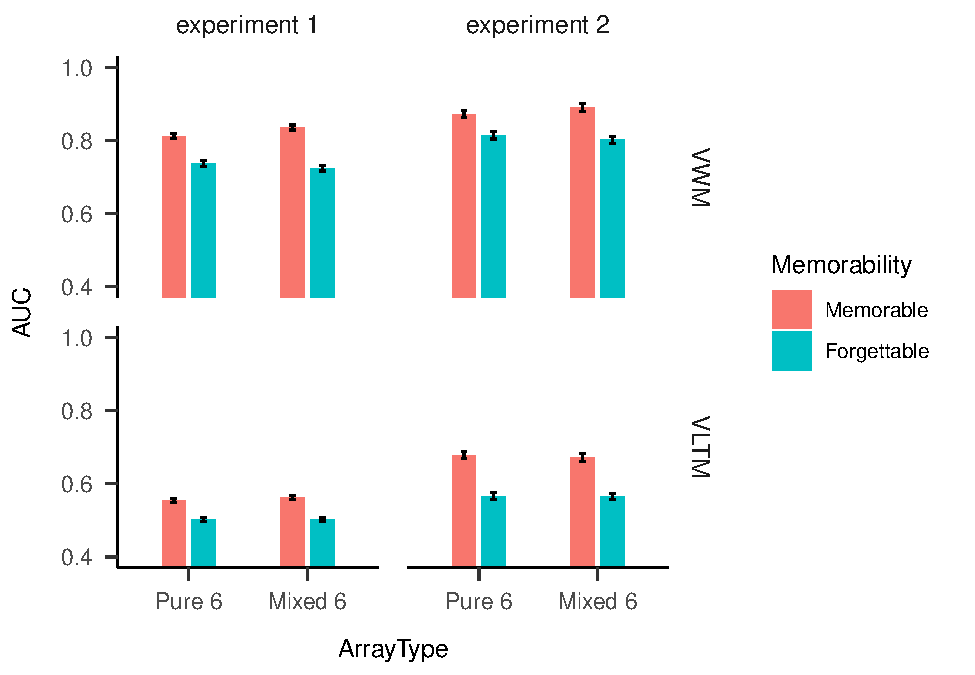
\includegraphics{Script_Re_Greer_2023_group1Rock_2023_files/figure-latex/plot for competitive hypothesis-1.pdf}
Our results are identical to the original results.

In both Experiment 1 and Experiment 2, memorable stimuli had higher Area Under the Curve (AUC) values compared to forgettable stimuli in both the Visual Working Memory (VWM) and Very Long-Term Memory (VLTM) tasks.

Notably, there was a significant interaction between memorability and array type in VWM. When memorable stimuli were encoded with forgettable stimuli, the VWM performance for memorable stimuli was higher compared to when all stimuli were memorable. This finding supports the competitiveness hypothesis.

However, this competitive advantage did not transfer to VLTM, as there was no main effect of array type or interaction between array type and memorability in VLTM.

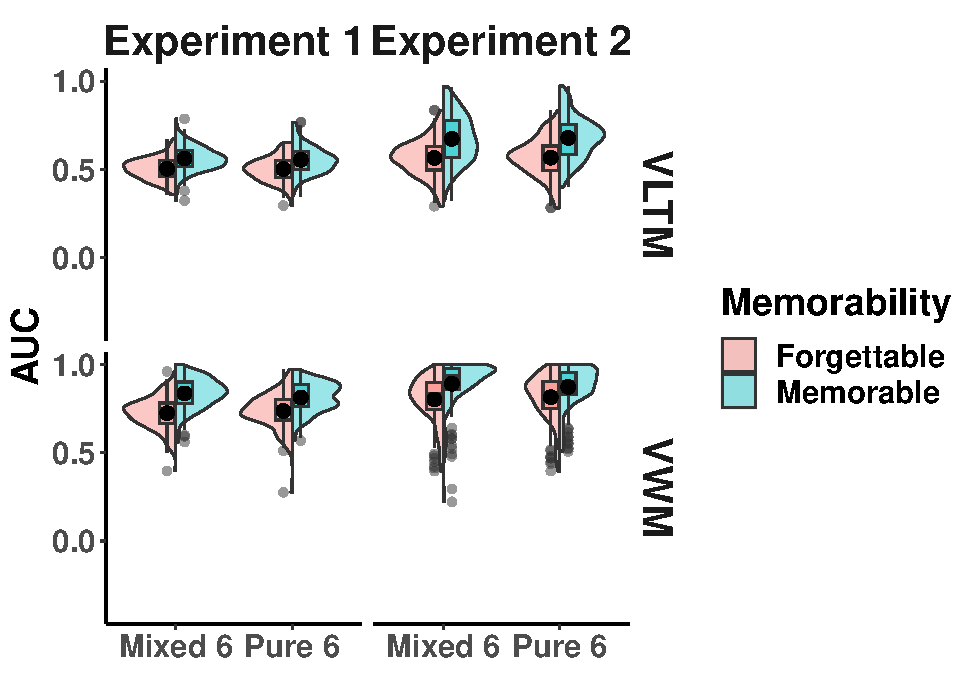
\includegraphics{Script_Re_Greer_2023_group1Rock_2023_files/figure-latex/Split violin plots for competitive hypo-1.pdf}

\hypertarget{testing-the-stickiness-hypothesis-memorable-stimuli-are-stickier-than-forgettable-stimuli}{%
\subsection{Testing the stickiness hypothesis: memorable stimuli are stickier than forgettable stimuli}\label{testing-the-stickiness-hypothesis-memorable-stimuli-are-stickier-than-forgettable-stimuli}}

since the author didn't explicitly mention the recoding job in paper, to ensure the recoding definitely exists, here we show the anova result of experiment1 -- 2 (ArrayType: Pure 3 and Pure 6) × 2 (Memorability: Memorable and Forgettable) repeated measures ANOVA on stickiness, for convenience, this is the only replication result. next we will use the original data(without recoding) to do data analysis.

\begin{verbatim}
## 
## ====== ANOVA (Within-Subjects Design) ======
## 
## Descriptives:
## ────────────────────────────
##  "A_" "B_"  Mean    S.D.   n
## ────────────────────────────
##  SS3. Forg 0.113 (0.155) 156
##  SS3. Mem  0.317 (0.167) 156
##  SS6. Forg 0.141 (0.228) 156
##  SS6. Mem  0.211 (0.223) 156
## ────────────────────────────
## Total sample size: N = 156
## 
## ANOVA Table:
## Dependent variable(s):      A_SS3&B_Forg, A_SS3&B_Mem, A_SS6&B_Forg, A_SS6&B_Mem
## Between-subjects factor(s): –
## Within-subjects factor(s):  A_, B_
## Covariate(s):               –
## ──────────────────────────────────────────────────────────────────────
##             MS   MSE df1 df2      F     p     η²p [90% CI of η²p]  η²G
## ──────────────────────────────────────────────────────────────────────
## A_       0.237 0.035   1 155  6.708  .011 *     .041 [.005, .104] .010
## B_       2.932 0.042   1 155 69.938 <.001 ***   .311 [.216, .400] .110
## A_ * B_  0.696 0.031   1 155 22.782 <.001 ***   .128 [.057, .213] .028
## ──────────────────────────────────────────────────────────────────────
## MSE = mean square error (the residual variance of the linear model)
## η²p = partial eta-squared = SS / (SS + SSE) = F * df1 / (F * df1 + df2)
## ω²p = partial omega-squared = (F - 1) * df1 / (F * df1 + df2 + 1)
## η²G = generalized eta-squared (see Olejnik & Algina, 2003)
## Cohen’s f² = η²p / (1 - η²p)
## 
## Levene’s Test for Homogeneity of Variance:
## No between-subjects factors. No need to do the Levene’s test.
## 
## Mauchly’s Test of Sphericity:
## The repeated measures have only two levels. The assumption of sphericity is always met.
\end{verbatim}

\begin{verbatim}
## 
## ====== ANOVA (Within-Subjects Design) ======
## 
## Descriptives:
## ────────────────────────────
##  "A_" "B_"  Mean    S.D.   n
## ────────────────────────────
##  SS3. Forg 0.071 (0.198) 156
##  SS3. Mem  0.315 (0.171) 156
##  SS6. Forg 0.021 (0.684) 156
##  SS6. Mem  0.168 (0.329) 156
## ────────────────────────────
## Total sample size: N = 156
## 
## ANOVA Table:
## Dependent variable(s):      A_SS3&B_Forg, A_SS3&B_Mem, A_SS6&B_Forg, A_SS6&B_Mem
## Between-subjects factor(s): –
## Within-subjects factor(s):  A_, B_
## Covariate(s):               –
## ──────────────────────────────────────────────────────────────────────
##             MS   MSE df1 df2      F     p     η²p [90% CI of η²p]  η²G
## ──────────────────────────────────────────────────────────────────────
## A_       1.515 0.149   1 155 10.188  .002 **    .062 [.015, .132] .015
## B_       5.952 0.147   1 155 40.571 <.001 ***   .207 [.121, .298] .056
## A_ * B_  0.365 0.123   1 155  2.975  .087 .     .019 [.000, .068] .004
## ──────────────────────────────────────────────────────────────────────
## MSE = mean square error (the residual variance of the linear model)
## η²p = partial eta-squared = SS / (SS + SSE) = F * df1 / (F * df1 + df2)
## ω²p = partial omega-squared = (F - 1) * df1 / (F * df1 + df2 + 1)
## η²G = generalized eta-squared (see Olejnik & Algina, 2003)
## Cohen’s f² = η²p / (1 - η²p)
## 
## Levene’s Test for Homogeneity of Variance:
## No between-subjects factors. No need to do the Levene’s test.
## 
## Mauchly’s Test of Sphericity:
## The repeated measures have only two levels. The assumption of sphericity is always met.
\end{verbatim}

\begin{verbatim}
## 
## ====== ANOVA (Within-Subjects Design) ======
## 
## Descriptives:
## ────────────────────────────
##  "A_" "B_"  Mean    S.D.   n
## ────────────────────────────
##  SS3. Forg 0.361 (0.706) 156
##  SS3. Mem  0.660 (0.341) 156
##  SS6. Forg 0.232 (1.573) 156
##  SS6. Mem  0.483 (0.602) 156
## ────────────────────────────
## Total sample size: N = 156
## 
## ANOVA Table:
## Dependent variable(s):      A_SS3&B_Forg, A_SS3&B_Mem, A_SS6&B_Forg, A_SS6&B_Mem
## Between-subjects factor(s): –
## Within-subjects factor(s):  A_, B_
## Covariate(s):               –
## ───────────────────────────────────────────────────────────────────────
##              MS   MSE df1 df2      F     p     η²p [90% CI of η²p]  η²G
## ───────────────────────────────────────────────────────────────────────
## A_        3.682 0.885   1 155  4.160  .043 *     .026 [.000, .081] .007
## B_       11.803 0.882   1 155 13.376 <.001 ***   .079 [.024, .155] .022
## A_ * B_   0.089 0.848   1 155  0.105  .746       .001 [.000, .021] .000
## ───────────────────────────────────────────────────────────────────────
## MSE = mean square error (the residual variance of the linear model)
## η²p = partial eta-squared = SS / (SS + SSE) = F * df1 / (F * df1 + df2)
## ω²p = partial omega-squared = (F - 1) * df1 / (F * df1 + df2 + 1)
## η²G = generalized eta-squared (see Olejnik & Algina, 2003)
## Cohen’s f² = η²p / (1 - η²p)
## 
## Levene’s Test for Homogeneity of Variance:
## No between-subjects factors. No need to do the Levene’s test.
## 
## Mauchly’s Test of Sphericity:
## The repeated measures have only two levels. The assumption of sphericity is always met.
\end{verbatim}

\begin{verbatim}
## 
## ====== ANOVA (Within-Subjects Design) ======
## 
## Descriptives:
## ──────────────────────────────
##    "A_" "B_"  Mean    S.D.   n
## ──────────────────────────────
##  Mixed. Forg 0.399 (1.990) 156
##  Mixed. Mem  0.413 (0.868) 156
##  SS6.   Forg 0.232 (1.573) 156
##  SS6.   Mem  0.483 (0.602) 156
## ──────────────────────────────
## Total sample size: N = 156
## 
## ANOVA Table:
## Dependent variable(s):      A_Mixed&B_Forg, A_Mixed&B_Mem, A_SS6&B_Forg, A_SS6&B_Mem
## Between-subjects factor(s): –
## Within-subjects factor(s):  A_, B_
## Covariate(s):               –
## ─────────────────────────────────────────────────────────────────────
##             MS   MSE df1 df2     F     p     η²p [90% CI of η²p]  η²G
## ─────────────────────────────────────────────────────────────────────
## A_       0.369 1.719   1 155 0.215  .644       .001 [.000, .026] .000
## B_       2.759 1.977   1 155 1.396  .239       .009 [.000, .049] .002
## A_ * B_  2.177 1.928   1 155 1.129  .290       .007 [.000, .045] .002
## ─────────────────────────────────────────────────────────────────────
## MSE = mean square error (the residual variance of the linear model)
## η²p = partial eta-squared = SS / (SS + SSE) = F * df1 / (F * df1 + df2)
## ω²p = partial omega-squared = (F - 1) * df1 / (F * df1 + df2 + 1)
## η²G = generalized eta-squared (see Olejnik & Algina, 2003)
## Cohen’s f² = η²p / (1 - η²p)
## 
## Levene’s Test for Homogeneity of Variance:
## No between-subjects factors. No need to do the Levene’s test.
## 
## Mauchly’s Test of Sphericity:
## The repeated measures have only two levels. The assumption of sphericity is always met.
\end{verbatim}

\begin{verbatim}
## 
## ====== ANOVA (Within-Subjects Design) ======
## 
## Descriptives:
## ──────────────────────────────
##    "A_" "B_"  Mean    S.D.   n
## ──────────────────────────────
##  Mixed. Forg 0.337 (4.323) 156
##  Mixed. Mem  0.192 (0.289) 156
##  SS6.   Forg 0.021 (0.684) 156
##  SS6.   Mem  0.168 (0.329) 156
## ──────────────────────────────
## Total sample size: N = 156
## 
## ANOVA Table:
## Dependent variable(s):      A_Mixed&B_Forg, A_Mixed&B_Mem, A_SS6&B_Forg, A_SS6&B_Mem
## Between-subjects factor(s): –
## Within-subjects factor(s):  A_, B_
## Covariate(s):               –
## ─────────────────────────────────────────────────────────────────────
##             MS   MSE df1 df2     F     p     η²p [90% CI of η²p]  η²G
## ─────────────────────────────────────────────────────────────────────
## A_       4.504 5.076   1 155 0.887  .348       .006 [.000, .041] .001
## B_       0.000 4.383   1 155 0.000  .996       .000 [.000, .000] .000
## A_ * B_  3.335 4.540   1 155 0.735  .393       .005 [.000, .039] .001
## ─────────────────────────────────────────────────────────────────────
## MSE = mean square error (the residual variance of the linear model)
## η²p = partial eta-squared = SS / (SS + SSE) = F * df1 / (F * df1 + df2)
## ω²p = partial omega-squared = (F - 1) * df1 / (F * df1 + df2 + 1)
## η²G = generalized eta-squared (see Olejnik & Algina, 2003)
## Cohen’s f² = η²p / (1 - η²p)
## 
## Levene’s Test for Homogeneity of Variance:
## No between-subjects factors. No need to do the Levene’s test.
## 
## Mauchly’s Test of Sphericity:
## The repeated measures have only two levels. The assumption of sphericity is always met.
\end{verbatim}

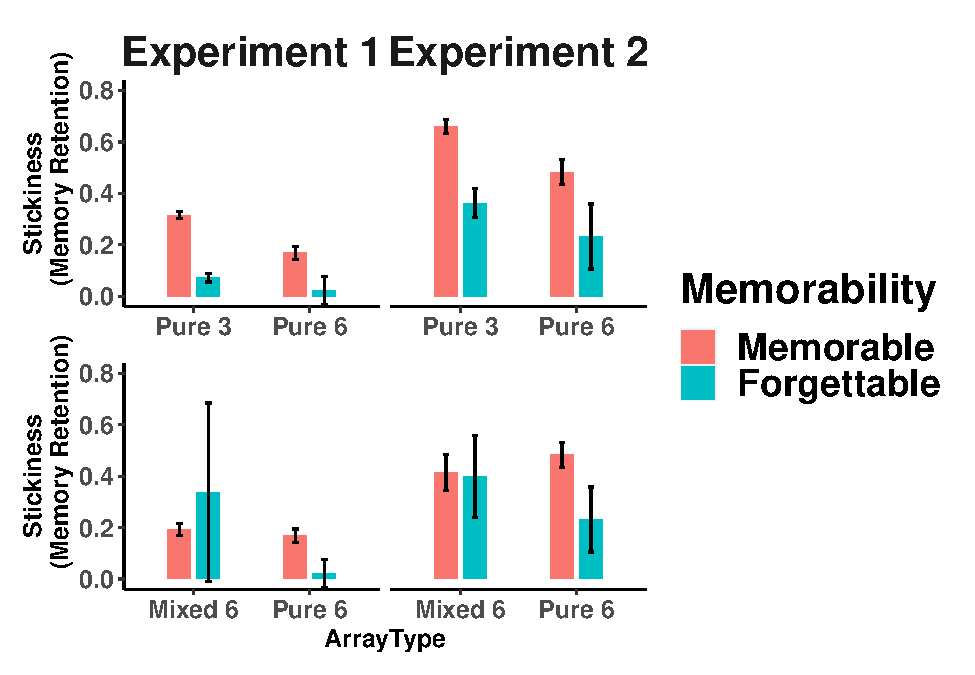
\includegraphics{Script_Re_Greer_2023_group1Rock_2023_files/figure-latex/paste top and bottom-1.pdf}

\begin{verbatim}
## Warning: Removed 9 rows containing non-finite values (`stat_ydensity()`).
\end{verbatim}

\begin{verbatim}
## Warning: Removed 9 rows containing non-finite values (`stat_boxplot()`).
\end{verbatim}

\begin{verbatim}
## Warning: Removed 9 rows containing non-finite values (`stat_summary()`).
\end{verbatim}

\begin{verbatim}
## Warning: Removed 15 rows containing non-finite values (`stat_ydensity()`).
\end{verbatim}

\begin{verbatim}
## Warning: Removed 15 rows containing non-finite values (`stat_boxplot()`).
\end{verbatim}

\begin{verbatim}
## Warning: Removed 15 rows containing non-finite values (`stat_summary()`).
\end{verbatim}

\begin{verbatim}
## Warning: Removed 115 rows containing missing values (`geom_split_violin()`).
\end{verbatim}

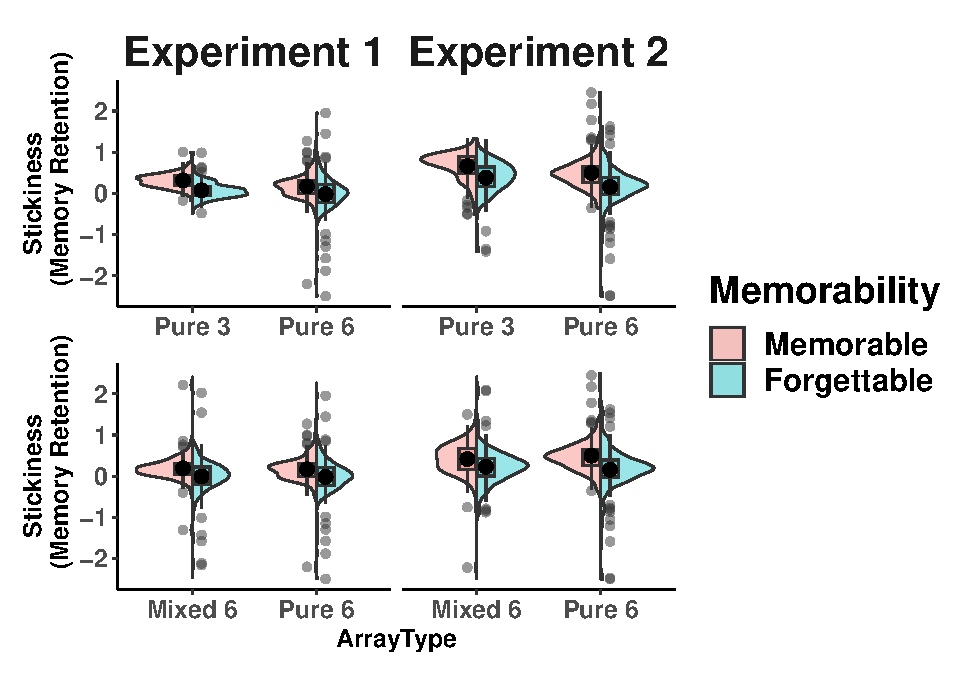
\includegraphics{Script_Re_Greer_2023_group1Rock_2023_files/figure-latex/unnamed-chunk-17-1.pdf}

\hypertarget{discussion}{%
\section{Discussion}\label{discussion}}

\hypertarget{efficiency-benefit}{%
\subsection{Efficiency benefit}\label{efficiency-benefit}}

For the efficiency benefit of memorable stimuli, memorable stimuli benefit from existing long-term memory representations.Existing long-term memory representations can assist working memory performance by reducing the need for active maintenance of stimuli in visual working memory.

Also, the hypothesis does not fully explain the findings because both memorable and forgettable stimuli were presented equally in the experiments.Memorable and forgettable. Future studies should explore cognitive mechanisms that allow efficient representations of novel but memorable stimuli.

\hypertarget{competitive-benefit}{%
\subsection{Competitive benefit}\label{competitive-benefit}}

we speculate that differences in attentional allocation during encoding might play a role in this competitive advantage. memorable stimuli are more likely to attract attention, leading to the observed competitive advantage in VWM.

However, it remains unclear what specifically attracts attention to memorable stimuli. A recent study by (Bainbridge, 2020)suggests that perceptual saliency is unlikely to be the sole factor, as memorable stimuli do not capture attention in a stimulus-driven manner. Therefore, attentional allocation differences between memorable and forgettable stimuli are likely to occur post-perceptually.

Importantly, while the competitive benefit was observed in VWM, it did not translate into VLTM. Therefore, although memorable stimuli may attract more attention, attentional allocation alone does not fully explain their memorability.

\hypertarget{stickiness}{%
\subsection{Stickiness}\label{stickiness}}

The study's findings indicate that memorable stimuli are more ``stickier'' or better retained in visual working memory (VWM) compared to forgettable stimuli. However, the underlying mechanisms that produce the memorability benefit within VWM and the stickiness benefit might be dissociable. Recent research suggests that despite differences in VWM capacity, the rate at which information remains in very long-term memory (VLTM) is comparable between young adults and school-aged children, indicating dissociable mechanisms(Forsberg, Guitard, Adams, Pattanakul, \& Cowan, 2022). Moreover, the rate of encoding into VWM can be independent of the rate of forgetting.

Future research should investigate whether the mechanisms leading to memorability and stickiness benefits are distinct and how memorable stimuli resist interference or better consolidate in VWM, potentially through robust decay resistance or a combination of both factors. Additional studies are needed to shed light on the developmental aspects of the stickiness of memorable and forgettable stimuli.

\newpage

\hypertarget{references}{%
\section{References}\label{references}}

\hypertarget{refs}{}
\begin{CSLReferences}{1}{0}
\leavevmode\vadjust pre{\hypertarget{ref-R-papaja}{}}%
Aust, F., \& Barth, M. (2022). \emph{{papaja}: {Prepare} reproducible {APA} journal articles with {R Markdown}}. Retrieved from \url{https://github.com/crsh/papaja}

\leavevmode\vadjust pre{\hypertarget{ref-bainbridge_resiliency_2020}{}}%
Bainbridge, W. A. (2020). The resiliency of image memorability: {A} predictor of memory separate from attention and priming. \emph{Neuropsychologia}, \emph{141}, 107408. \url{https://doi.org/10.1016/j.neuropsychologia.2020.107408}

\leavevmode\vadjust pre{\hypertarget{ref-bainbridge_intrinsic_2013}{}}%
Bainbridge, W. A., Isola, P., \& Oliva, A. (2013). The {Intrinsic} {Memorability} of {Face} {Photographs}. \emph{JOURNAL OF EXPERIMENTAL PSYCHOLOGY-GENERAL}, \emph{142}(4), 1323--1334. \url{https://doi.org/10.1037/a0033872}

\leavevmode\vadjust pre{\hypertarget{ref-R-bruceR}{}}%
Bao, H.-W.-S. (2023). \emph{bruceR: Broadly useful convenient and efficient r functions}. Retrieved from \url{https://CRAN.R-project.org/package=bruceR}

\leavevmode\vadjust pre{\hypertarget{ref-forsberg_childrens_2022}{}}%
Forsberg, A., Guitard, D., Adams, E. J., Pattanakul, D., \& Cowan, N. (2022). Children's long-term retention is directly constrained by their working memory capacity limitations. \emph{Developmental Science}, \emph{25}(2), e13164. \url{https://doi.org/10.1111/desc.13164}

\leavevmode\vadjust pre{\hypertarget{ref-isola_what_2014}{}}%
Isola, P., Xiao, J., Parikh, D., Torralba, A., \& Oliva, A. (2014). What {Makes} a {Photograph} {Memorable}? \emph{IEEE Transactions on Pattern Analysis and Machine Intelligence}, \emph{36}(7), 1469--1482. \url{https://doi.org/10.1109/TPAMI.2013.200}

\leavevmode\vadjust pre{\hypertarget{ref-R-bayestestR}{}}%
Makowski, D., Ben-Shachar, M. S., \& Lüdecke, D. (2019). bayestestR: Describing effects and their uncertainty, existence and significance within the bayesian framework. \emph{Journal of Open Source Software}, \emph{4}(40), 1541. \url{https://doi.org/10.21105/joss.01541}

\leavevmode\vadjust pre{\hypertarget{ref-R-patchwork}{}}%
Pedersen, T. L. (2022). \emph{Patchwork: The composer of plots}. Retrieved from \url{https://CRAN.R-project.org/package=patchwork}

\leavevmode\vadjust pre{\hypertarget{ref-R-base}{}}%
R Core Team. (2023). \emph{R: A language and environment for statistical computing}. Vienna, Austria: R Foundation for Statistical Computing. Retrieved from \url{https://www.R-project.org/}

\leavevmode\vadjust pre{\hypertarget{ref-saito_judgments_2023}{}}%
Saito, J. M., Kolisnyk, M., \& Fukuda, K. (2023). Judgments of learning reveal conscious access to stimulus memorability. \emph{PSYCHONOMIC BULLETIN \& REVIEW}, \emph{30}(1), 317--330. \url{https://doi.org/10.3758/s13423-022-02166-1}

\leavevmode\vadjust pre{\hypertarget{ref-R-ggplot2}{}}%
Wickham, H. (2016). \emph{ggplot2: Elegant graphics for data analysis}. Springer-Verlag New York. Retrieved from \url{https://ggplot2.tidyverse.org}

\leavevmode\vadjust pre{\hypertarget{ref-R-dplyr}{}}%
Wickham, H., François, R., Henry, L., Müller, K., \& Vaughan, D. (2023). \emph{Dplyr: A grammar of data manipulation}. Retrieved from \url{https://CRAN.R-project.org/package=dplyr}

\leavevmode\vadjust pre{\hypertarget{ref-R-tidyr}{}}%
Wickham, H., Vaughan, D., \& Girlich, M. (2023). \emph{Tidyr: Tidy messy data}. Retrieved from \url{https://CRAN.R-project.org/package=tidyr}

\end{CSLReferences}


\end{document}
